\documentclass[a4paper, 12pt]{article}
\usepackage[dvipsnames]{xcolor}
\usepackage{float, subfigure, graphicx, grffile, textcomp}
\usepackage{indentfirst}
\usepackage{enumerate}
\usepackage{fancyhdr}
\usepackage{gensymb}
\usepackage{geometry}
\setlength{\headheight}{32.09pt}
\renewcommand{\contentsname}{Sumário}
\renewcommand{\figurename}{Figura}
\renewcommand{\tablename}{Tabela}
% \renewcommand{\footrulewidth}{0.2pt} # insere uma linha no rodapé da página
\setlength{\parskip}{0.25cm}

\geometry{a4paper, left=2.5cm, right=2cm, top=3cm, bottom=3cm}

\begin{document}

\pagenumbering{gobble}


%CAPA~~~~~~~~~~~~


\title{\textbf{Universidade de São Paulo\\ Escola Politécnica}
	\vspace{15pt}
	\begin{figure}[!h]
		\centering
		
\includegraphics[scale=0.15]{Poli}
	\end{figure}
	\vspace{30pt}
	\\\textbf{MAP3121: Métodos Numéricos e Aplicações} \\
	\vspace{15pt} {Exercício Programa 1}\\
	\vspace{10pt}
	\vspace{15pt} 
	\Large{Turmas 05 e 06: Professor Claudio Hirofume Asano}}


	\author{Guilherme Fernandes Alves - 10774361 \\ Ricardo Aguiar de Andrade - 10774674 \vspace{85pt}}
	\date{\textbf{\Large{São Paulo, Abril de 2020}}}
	\maketitle


\thispagestyle{empty}
\newpage

%FIM DA CAPA~~~~~~~~~~~~

%SUMÁRIO~~~~~~~~~~~~

\tableofcontents
\thispagestyle{empty}
\newpage

%FIM DO SUMÁRIO~~~~~~~~~~~~


%INTRODUÇÃO~~~~~~~~~~~~
\pagestyle{fancy}
\fancyhead[R]{\textcolor{gray}{\textit{Métodos Numéricos e Aplicações}}}
\lhead{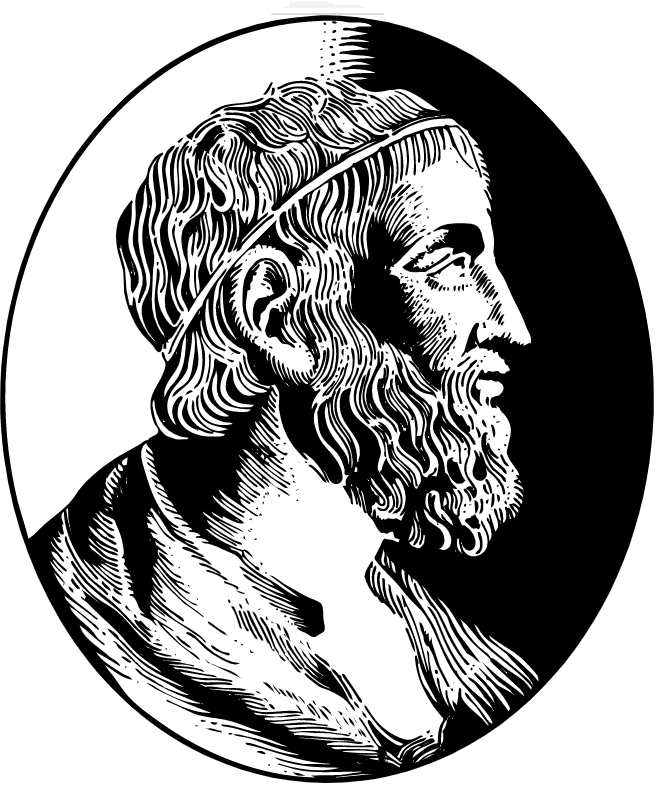
\includegraphics[scale=0.055]{ime}}
\pagenumbering{arabic}

\section{Resumo, objetivos e considerações iniciais}

O primeiro exercício programa (EP) da disciplina \textit{MAP3121 - Métodos Numéricos e Aplicações} se refere à resolução de um \textbf{problema direto} ligado à equação do calor. O problema se trata da determinação da distribuição de temperatura em uma barra sujeita a fontes de calor, a partir de uma dada distribuição inicial (condição de contorno). Este relatório consistirá de uma análise dos resultados obtidos para diferentes condições de contorno, bem como para diferentes fontes de calor a partir de parâmetros que serão inseridos pelo usuário. 

Todos os resultados serão gerados por um programa criado, em linguagem de programação \textit{Python 3}, pela dupla que vos escreve. O programa foi desenvolvido com base na teoria descrita no enunciado deste EP, assim como nos conhecimentos da dupla adquiridos ao longo da disciplina e além desta. O software é totalmente autêntico, sendo reconhecido todo o auxílio dos monitores da disciplina, bem como as informações retiradas do enunciado do EP. 

Para a realização do programa foram utilizadas funções inerentes à linguagem \textit{Python} e bibliotecas permitidas pela disciplina, tais como \textit{numpy} e \textit{matplotlib}. Também houve a utilização de duas variáveis globais, \textit{'n'} e \textit{'gr'}, visando uma compactação e facilidade de entendimento no código fonte, pois caso essas variáveis não fossem globais, algumas funções presentes no software teriam argumentos inutilizáveis, visto que dependendo do teste a ser realizado, \textit{'n'} pode ou não ser necessária para os cálculos em determinadas funções. Por fim, o software foi escrito no ambiente de desenvolvimento integrado (IDE) \textit{PyCharm}, em versão comunitária. 

Este relatório tem como objetivos interpretar e analisar os resultados obtidos a partir do exercício programa proposto, com ênfase no comportamento do erro para os diversos casos solicitados pelo enunciado. Além disso, busca-se um entendimento dos diferentes comportamentos do software de acordo com cada método implementado (Euler explícito, Euler implícito ou Crank-Nicolson) para aproximar a equação do calor, destacando as principais diferenças entre cada método.


%FIM DA INTRODUÇÃO~~~~~~~~~~~~


%CORPO PRINCIPAL~~~~~~~~~~~
\section{Fundamentos Teóricos}

Conforme enunciado do EP, a evolução da distribuição de temperatura em uma barra é dada pela seguinte equação diferencial parcial:

\begin{equation}u_{t}(t,x)=u_{xx}(t,x)+f(t,x) \hspace{0.2cm}em\hspace{0.2cm} [0,T] \times [0,1]\end{equation}

Sendo as condições de contorno dadas por:

\begin{eqnarray}
u(0,x) & = & u_{0}(x) \hspace{0.2cm}em\hspace{0.2cm} [0,1]\\
u(t,0) & = & g_{1}(t) \hspace{0.2cm}em\hspace{0.2cm} [0,T]\\
u(t,1) & = & g_{2}(t) \hspace{0.2cm}em\hspace{0.2cm} [0,T]
\end{eqnarray}

Onde $t$ é a variável temporal e $x$ a variável espacial. Usa-se a seguinte notação compacta para as derivadas parciais:

$$u_{xx}(t,x)=\frac{\partial^{2}u(t,x)}{\partial x^2}$$

O comprimento da barra foi normalizado para $1$ e integrar-se-á a equação num intervalo de tempo de $0$ a $T$. A variável $u(t,x)$ descreve a temperatura no instante $t$ e na posição $x$. Nota-se que as condições de contorno (3) e (4) denotam-se condições de fronteira, enquanto a condição (2) trata-se da temperatura no instante inicial para cada posição $x$. A função $f$ descreve as fontes de calor ao longo do tempo.

\subsection{Discretizações da equação do calor}

Desejamos aproximar numericamente a solução de (1)-(4). Para isso, vamos aproximar as derivadas parciais pelo método das \textit{diferenças finitas}, que são baseadas em expansões de Taylor. 

Para a discretização da equação do calor introduzir-se-á uma malha espacial dada pelos pontos $x_{i} = i\Delta x$, $i=0, \dots ,N$, com $\Delta x=\frac{1}{N}$. Para a discretização temporal definimos $\Delta t =\frac{T}{M}$, e calculamos aproximações nos instantes $t_{k}=k\Delta t$, $k=1, \dots,M$. Denotaremos a aproximação para a solução nos pontos de malha $u(t_{k},x_{i})$ por $u_{i}^k$. 

Desta forma teremos a condição inicial dada por:

$$ u_{i}^0	= u_{0}(x_{i}), \hspace{0.2cm} i=0,\cdots,N	$$

Ao longo da evolução temporal as condições de fronteira são dadas por:

$$ u_{0}^k	= g_{1}(t_{k}) \hspace{0.2cm} e \hspace{0.2cm} u_{N}^k	= g_{2}(t_{k}), \hspace{0.2cm} k=1,\cdots,M	$$

Para os pontos interiores a evolução é aproximada pelas fórmulas de diferenças finitas:

\begin{eqnarray}
u_{i}^{k+1} & = & u_{i}^{k} + \Delta t (\frac{u_{i-1}^{k}-2u_{i}^{k}+u_{i+1}^{k}}{\Delta x^2}+f(x_i,t_k)), \hspace{0.2cm} i=1,\cdots,N-1, \hspace{0.2cm} k=0,\cdots,M-1 \hspace{1cm}
\end{eqnarray}

Dadas as condições de contorno do problema a expressão (5) permite a determinação da solução aproximada em todos os instantes e em todas as posições, computando sequencialmente desde $t_0=0$ a $t_M=T$. 

\textbf{Convergência da solução}

Conforme é demonstrado no enunciado do EP, se $u(t,x)$ possuir 4 derivadas contínuas em $x$ e duas em $t$ no domínio de integração $D=[0,T] \times [0,1]$ o erro de truncamento $\tau$ converge a zero quando $\Delta t$ e $\Delta x$ tendem a zero. No entanto, o que realmente queremos é que a solução aproximada nos pontos de malha convirja para a solução exata da equação do calor. Vamos definir o erro entre a solução aproximada e a exata da seguinte forma:

\begin{equation}
e_i^k = u(t_k,x_i) - u_i^k
\end{equation}

Sendo a norma do erro no instante $t_k$ dada por:

\begin{equation}
\|e^k\| = \max_{i}|e_i^k| 
\end{equation}

É possível demonstrar, conforme enunciado do EP, que, se tomarmos $\lambda = \frac{\Delta t}{\Delta x^2}$, o erro $e_i^k$ tende a zero quando $\lambda \leq \frac{1}{2}$. Neste caso, dizemos que a solução aproximada converge para a solução exata da equação do calor. 

Caso esta condição seja violada o método fica instável, com o erro se amplificando enormemente. Este método é dito \textit{condicionalmente convergente} de ordem 2 em $\Delta x$.

\subsection{Método implícito}

Até o momento, tudo o que foi discutido anteriormente, com o método (5), se trata de um método explícito, isto é, a solução em cada ponto em um novo instante de tempo é obtida simplesmente avaliando uma combinação de valores vizinhos do passo anterior. Já em um método implícito, a solução em um ponto
de malha no novo instante depende também de outros valores no mesmo instante, tornando-se necessário a solução de um sistema de equações a cada passo no tempo. Um exemplo disso é o método de Euler implícito, dado por:

\begin{eqnarray}
u_{i}^{k+1} & = & u_{i}^{k} + \lambda (u_{i-1}^{k+1} -2u_{i}^{k+1} +u_{i+1}^{k+1}) + \Delta t f(x_i,t_{k+1}), \hspace{0.2cm} i=1,\cdots,N-1, \hspace{0.2cm} k=0,\cdots,M-1 \hspace{1cm}
\end{eqnarray}


Neste método, para a evolução temporal, necessitamos resolver a cada passo um sistema linear com uma matriz $A$ tridiagonal simétrica:


\begin{equation}
\left[\begin{array}{ccccc}
	
	1+2\lambda   & -\lambda     & 0 		 & \cdots    	& 0 			\\ 
	-\lambda     & 1+2\lambda   & -\lambda   &  \ddots  	&  \vdots   	\\ 
	0 			 &  \ddots  	&  \ddots    &  \ddots  	& 0 			\\ 
	 \vdots  	 &  \ddots  	& - \lambda  & 1+2 \lambda  & - \lambda  	\\ 
	0 			 &  \cdots  	& 0 		 & - \lambda  	& 1+2 \lambda 
	
\end{array} \right] 
\left[\begin{array}{c}
u_{1}^{k+1} 			\\ 
u_{2}^{k+1} 			\\ 
\vdots 					\\ 
u_{N-2}^{k+1} 			\\ 
u_{N-1}^{k+1}
\end{array} \right] 
=
\left[\begin{array}{c}
u_{1}^k + \Delta t f_{1}^{k+1} + \lambda g_{1}(t^{k+1}) \\ 
u_{2}^k + \Delta t f_{2}^{k+1} 						 \\ 
\vdots 								 \\ 
u_{N-2}^k + \Delta t f_{N-2}^{k+1} 						 \\ 
u_{N-1}^k + \Delta t f_{N-1}^{k+1} + \lambda g_{2}(t^{k+1})
\end{array} \right] 
\end{equation}


O método de Euler implícito é incondicionalmente estável e convergente de ordem 2 em $\Delta x$ e ordem 1 em $\Delta t$. Assim, mesmo não sofrendo restrições de estabilidade, a precisão do esquema estará limitada pela escolha de $\Delta t$.

Outro exemplo de método implícito é o método de Crank-Nicolson, que também é incondicionalmente estável, mas tem convergência de ordem 2 em $\Delta x$ e $\Delta t$:


\begin{eqnarray}
u_{i}^{k+1} & = & u_{i}^{k} + \frac{\lambda}{2} ((u_{i-1}^{k+1} -2u_{i}^{k+1} +u_{i+1}^{k+1}) + (u_{i-1}^{k} -2u_{i}^{k} +u_{i+1}^{k})) + \frac{\Delta t}{2} (f(x_i,t_{k} + f(x_i,t_{k+1})),\nonumber \\ &&\hspace{3.5cm} i=1,\cdots,N-1, \hspace{0.2cm} k=0,\cdots,M-1 \hspace{1cm}
\end{eqnarray}

Analogamente ao método de Euler implícito resolve-se um sistema linear com uma matriz tridiagonal simétrica a cada passo:

\begin{equation}
\left[\begin{array}{ccccc}
	
	1+\lambda   & -\frac{\lambda}{2}     & 0 		 & \cdots    	& 0 			\\ 
	-\frac{\lambda}{2}     & 1+\lambda   & -\frac{\lambda}{2}   &  \ddots  	&  \vdots   	\\ 
	0 			 &  \ddots  	&  \ddots    &  \ddots  	& 0 			\\ 
	 \vdots  	 &  \ddots  	& -\frac{\lambda}{2}  & 1+ \lambda  & -\frac{\lambda}{2}  	\\ 
	0 			 &  \cdots  	& 0 		 & -\frac{\lambda}{2}  	& 1+ \lambda 
	
\end{array} \right] 
\left[\begin{array}{c}
u_{1}^{k+1} 			\\ 
u_{2}^{k+1} 			\\ 
\vdots 					\\ 
u_{N-2}^{k+1} 			\\ 
u_{N-1}^{k+1}
\end{array} \right]
=
\end{equation}
$$= \left[\begin{array}{c}
u_{1}^k + \frac{\lambda}{2}(u_{0}^k -2u_{1}^k +u_{2}^k) +\frac{\Delta t}{2}(f_{1}^{k}+f_{1}^{k+1}) + \frac{\lambda}{2} g_{1}(t^{k+1}) \\ 
u_{2}^k +\frac{\lambda}{2}(u_{1}^k -2u_{2}^k +u_{3}^k) +\frac{\Delta t}{2}( f_{2}^{k}+f_{2}^{k+1}) \\ 
\vdots \\ 
u_{N-2}^k +\frac{\lambda}{2}(u_{N-3}^k -2u_{N-2}^k +u_{N-1}^k) +\frac{\Delta t}{2}( f_{N-2}^{k}+f_{N-2}^{k+1}) \\ 
u_{N-1}^k + \frac{\lambda}{2}(u_{N-2}^k -2u_{N-1}^k +u_{N}^k) + \frac{\Delta t}{2}( f_{N-1}^{k}+f_{N-1}^{k+1}) +\frac{\lambda}{2} g_{2}(t^{k+1})
\end{array} \right] 
$$

As análises de convergência destes dois métodos implícitos podem ser encontradas no enunciado deste EP e no livro \textbf{Analysis of Numerical Methods, E. Isaacson and H. B. Keller} não sendo repetidas aqui.


\section{Respostas das Questões Propostas}

\subsection{Primeira tarefa}

Nesta primeira tarefa nos foi solicitada a implementação do método da discretização (5). Para isso, foi imaginada uma matriz $\Psi$, ilustrada abaixo, constituída dos valores $u(t_k, x_i)=u_i^k$ que aproximam a solução exata para um instante $t_k$ numa posição $x_i$ da barra, onde $x_i = i \Delta x$ e $t_k = k \Delta t$. As linhas da matriz $\Psi$ representam os instantes, variando de $k=0$ (primeira linha) até $k=M$ (última linha); já as colunas representam as posições, variando de $i=0$ (primeira coluna) até $i=N$ (última coluna). 

É importante notar que a primeira linha é determinada pela condição de contorno (2). Já a primeira e a última coluna, \textbf{a partir do instante $k=1$}, são determinadas pelas condições de contorno (3) e (4), respectivamente. 

Desse modo, os valores $u_i^k$ com $i=1, 2,\cdots, N-1$ e $k=1,2,\cdots, M$ são determinados pela equação (5).

Em tempo de execução o usuário determina os valores de $N$ e $\lambda$, sendo $M$ determinado a partir destes dois parâmetros pela fórmula:

$$M=\frac{N^{2}T}{\lambda}$$

\textbf{Obs.}: A fórmula acima é deduzida a partir das definições de $\Delta t$, $\Delta x$ e $\lambda$ supracitadas.

Tendo em vista a matriz $\Psi$, foram implementadas no código algumas funções específicas para preenchimento das condições de contorno. Cada elemento da matriz que não está na fronteira ou na condição inicial pode ser calculado, através do método (5), com base nestas condições de contorno. Em outras palavras, sendo definido um vetor $u_{old}$ de dimensão $N-1$ que contenha os valores $u_i^0$ (instante inicial), podemos utilizar (5) para criar um vetor $u_{new}$ contendo os valores $u_{i}^{1}$. A partir disso, $u_{old} = u_{new}$ e $u_{new}$ é calculado novamente com a fórmula (5), contendo os valores  $u_i^2$. Assim o método segue até $u_i^M$.

$$
\Psi = \left[ \begin{array}{ccccccc}
u_{0}^0 	& u_{1}^0 	  & u_{2}^0  	 & u_{3}^0  	& \dots  & u_{N-1}^0  	& u_{N}^0       \\  \\
u_{0}^1 	& u_{1}^1 	  & u_{2}^1  	 & u_{3}^1  	& \dots  & u_{N-1}^1  	& u_{N}^1       \\  \\
u_{0}^2 	& u_{1}^2 	  & u_{2}^2  	 & u_{3}^2  	& \dots  & u_{N-1}^2  	& u_{N}^2       \\  \\
u_{0}^3 	& u_{1}^3 	  & u_{2}^3  	 & u_{3}^3  	& \dots  & u_{N-1}^3  	& u_{N}^3       \\  \\
\vdots      & \vdots      & \vdots	     & \vdots       & \ddots & \vdots    	& \vdots        \\  \\
u_{0}^{M-1} & u_{1}^{M-1} & u_{2}^{M-1}  & u_{3}^{M-1}  & \dots  & u_{N-1}^{M-1}& u_{N}^{M-1}   \\  \\
u_{0}^{M}   & u_{1}^{M}   & u_{2}^{M}    & u_{3}^{M}    & \dots  & u_{N-1}^{M}  & u_{N}^{M}     \\  \\
\end{array} \right]_{(M+1) \times (N+1)} 
$$

É importante notar que os vetores estão se sobrepondo, isto é, não estamos salvando na memória todos os valores de temperatura para cada instante e posição. Isso porque nos interessa somente as temperaturas no último instante $u_i^M$, sendo que, para calcular este vetor de temperaturas, precisamos dar $M$ passos no tempo. Como os vetores não são salvos na memória tivemos que plotar os gráficos ($0.1s$ em $0.1s$) conforme o método fosse sendo realizado.

Nesta primeira tarefa foram propostas 3 diferentes situações a serem analisadas, uma para cada item ($a$, $b$ ou $c$). Em todos os 3 casos foi fixado o valor $T = 1$ e todos os resultados estão apresentados detalhadamente nos próximos tópicos.

\subsubsection{Item (a)}
No item $a$, primeiro utilizamos a fonte $f(t, x) = 10x^2({x-1}) -60xt + 20t$ com condições de contorno e fronteira nulas, isto é, $u(0,x) = u(t,0) = u(t,1) = 0$. Para estas condições constatamos a solução exata como $u(t, x) = 10tx^{2}({x-1})$ e calculamos as normas dos erros dadas pela fórmula (6) para o instante $t=1$. 

% Lambda igual a 0.5 e N igual a 160
\begin{figure}[H]
	\centering
	\subfigure [$t=0.1s$] {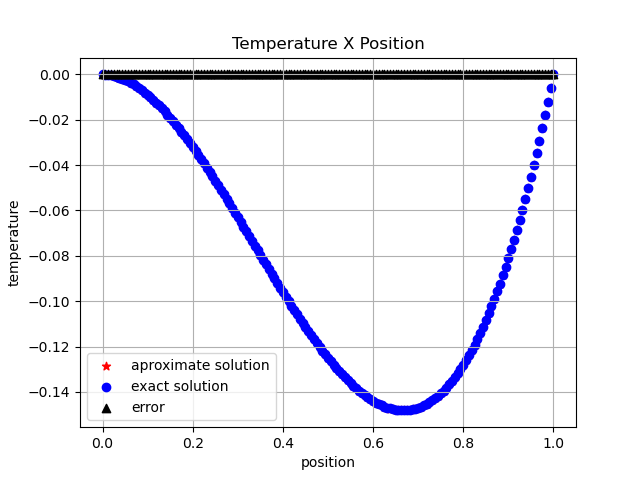
\includegraphics[scale=0.33]{graphs/aa_n_160_lambda_0.5/n_160_t_0.1_lambda_0.5.png}}
	\subfigure [$t=0.5s$] {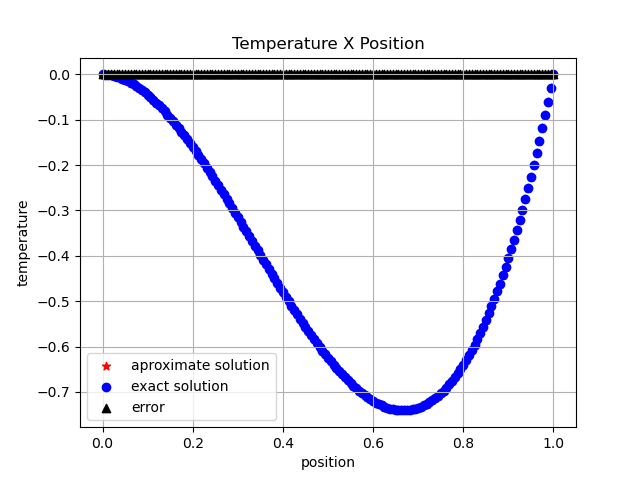
\includegraphics[scale=0.33]{graphs/aa_n_160_lambda_0.5/n_160_t_0.5_lambda_0.5.png}}
	\subfigure [$t=1.0s$] {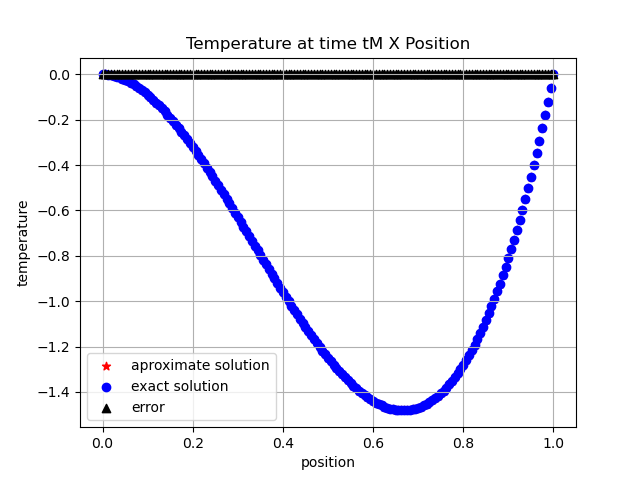
\includegraphics[scale=0.33]{graphs/aa_n_160_lambda_0.5/n_160_t_1.0_lambda_0.5.png}}
	\caption{\textit{$N = 160$, $\lambda$ = 0.5}}
\end{figure}

A tabela 1 apresenta resultados das normas dos erros em algumas das simulações.

% Colocar tabela com erros para cada simulação, com T=1, e diferentes resoluções de lambda
\begin{table}[!h]
    \centering
    \begin{tabular}{|c|c|c|c|}
    \hline                               % para uma linha horizontal
    N & Erro ($\lambda = 0.25$) & Erro ($\lambda = 0.50$) & Erro ($\lambda = 0.51$) \\
    \hline
    10  &  8.882e-16 & 4.441e-16 & 6.661e-16 \\
    20  &  1.554e-15 & 8.882e-16 & 7.143e-09 \\
    40  &  1.776e-15 & 1.332e-15 & 1.108e+31 \\
    80  &  1.177e-14 & 1.776e-15 & 8.545e+189 \\
    160 &  2.420e-14 & 2.666e-15 & $nan$ \\
    320 &  2.376e-14 & 1.332e-14 & $nan$ \\
    640 &  7.216e-14 & 5.040e-14 & $nan$ \\
    \hline
    \end{tabular}
    \caption{Norma do erro obtido em t = 1 para o item $a$.}
    %\label{tab:my_label}
\end{table}

Pelo fato das contas conterem aproximações, os erros para $\lambda \leq 0.5$ não resultam em 0 exatamente no instante $t=1$. Este fato faz com que o erro aumente à medida que $N$ aumenta, conforme é visto na tabela acima. Vale ressaltar que, na verdade, o erro não está aumentando verdadeiramente, esse aumento indevido é resultado das aproximações feitas durante os cálculos.

Em seguida nos foi dado a fonte:

$$f(t, x) = 10cos(10t)x^{2}(1-x)^{2}-(1+sin(10t))(12x^{2}-12x+2)$$

que corresponde à solução exata:

$$u(t, x) = (1+sin(10t))x^{2}(1-x)^{2}$$

com condições de contorno e fronteira:

$$u(0,x) = x^{2}(1-x)^{2} \hspace{0.25cm} e \hspace{0.25cm} u(t,0) = u(t,1) = 0$$

\textbf{Vamos denotar essas condições por "teste a"}.

Nessas condições foram requisitadas integrações com $N$ = 10, 20, 40, 80, 160, 320 e 640 para $\lambda = 0.5$, $\lambda = 0.25$ e $\lambda= 0.51$. Em seguida foi pedido para calcularmos o erro no instante $t=1$. As figuras de 2 à 22 apresentam os resultados obtidos com o código para as diferentes condições requisitadas. É possível acompanhar a evolução temporal da temperatura, obtida através da equação discretizada e da solução exata, assim como o erro dado pela fórmula (6).

% Lambda igual a 0.25 e N igual a 10
\begin{figure}[H]
	\centering
	\subfigure [$t=0.1s$] {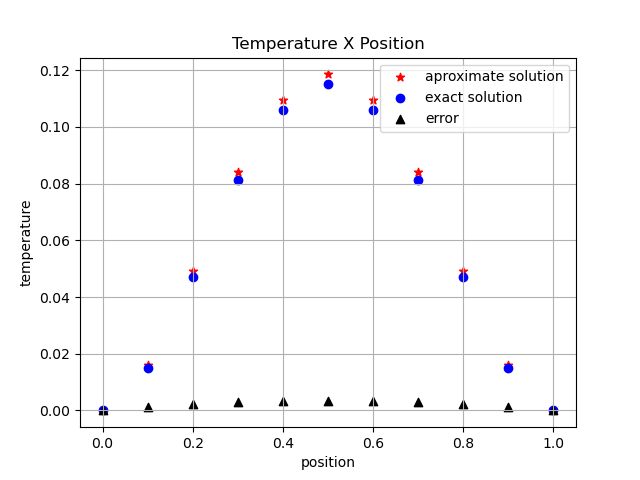
\includegraphics[scale=0.33]{graphs/a_n_10_lambda_0.25/n_10_t_0.1_lambda_0.25.png}}
	\subfigure [$t=0.5s$] {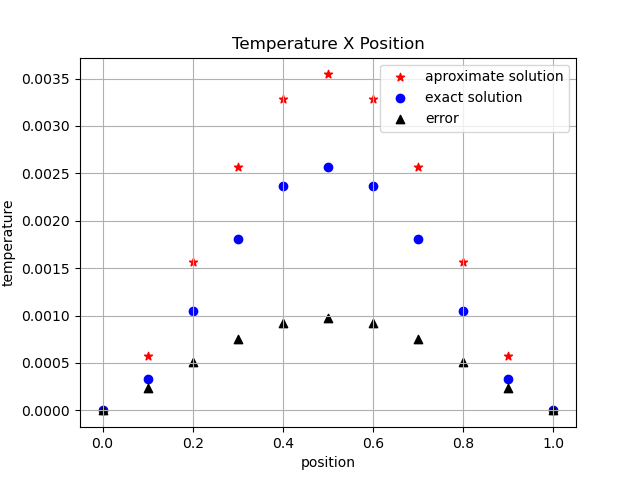
\includegraphics[scale=0.33]{graphs/a_n_10_lambda_0.25/n_10_t_0.5_lambda_0.25.png}}
	\subfigure [$t=1.0s$] {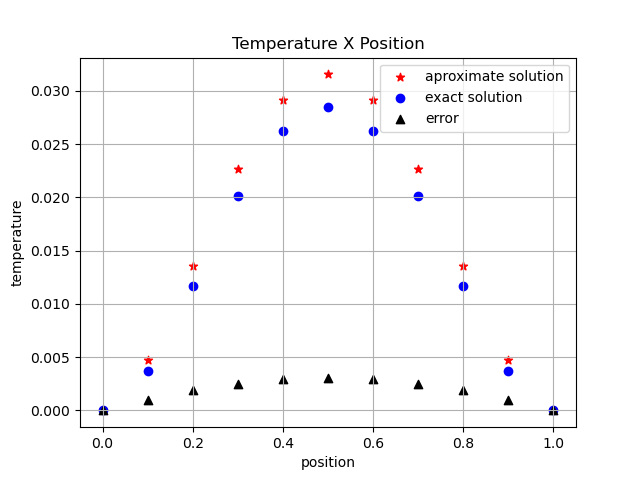
\includegraphics[scale=0.33]{graphs/a_n_10_lambda_0.25/n_10_t_1.0_lambda_0.25.png}}
	\caption{\textit{$N = 10$, $\lambda$ = 0.25}}
\end{figure}  

% Lambda igual a 0.25 e N igual a 20
\begin{figure}[H]
	\centering
    \subfigure [$t=0.1s$] {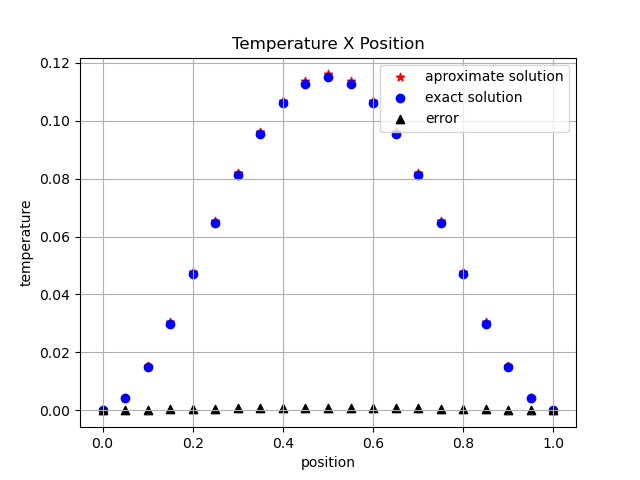
\includegraphics[scale=0.33]{graphs/a_n_20_lambda_0.25/n_20_t_0.1_lambda_0.25.png}}
	\subfigure [$t=0.5s$] {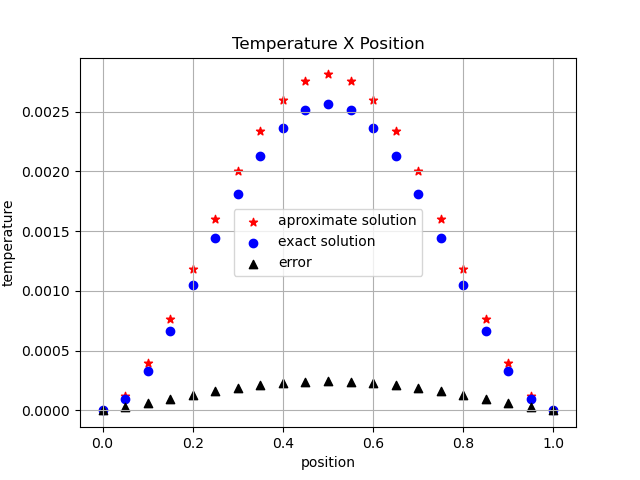
\includegraphics[scale=0.33]{graphs/a_n_20_lambda_0.25/n_20_t_0.5_lambda_0.25.png}}
	\subfigure [$t=1.0s$] {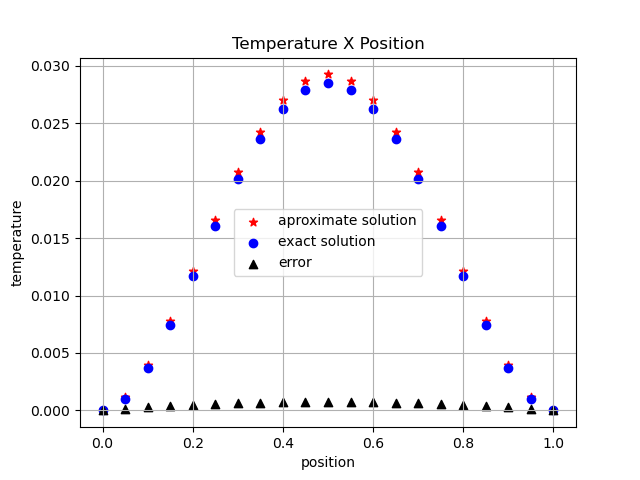
\includegraphics[scale=0.33]{graphs/a_n_20_lambda_0.25/n_20_t_1.0_lambda_0.25.png}}
	\caption{\textit{$N = 20$, $\lambda$ = 0.25}}
\end{figure}  

% Lambda igual a 0.25 e N igual a 40
\begin{figure}[H]
	\centering
	\subfigure [$t=0.1s$] {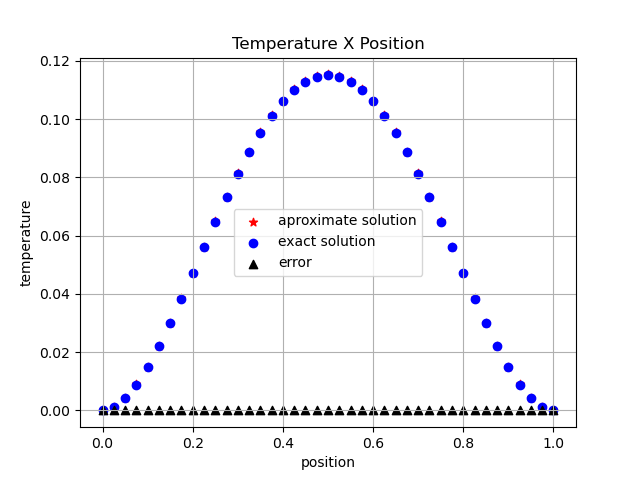
\includegraphics[scale=0.33]{graphs/a_n_40_lambda_0.25/n_40_t_0.1_lambda_0.25.png}}
	\subfigure [$t=0.5s$] {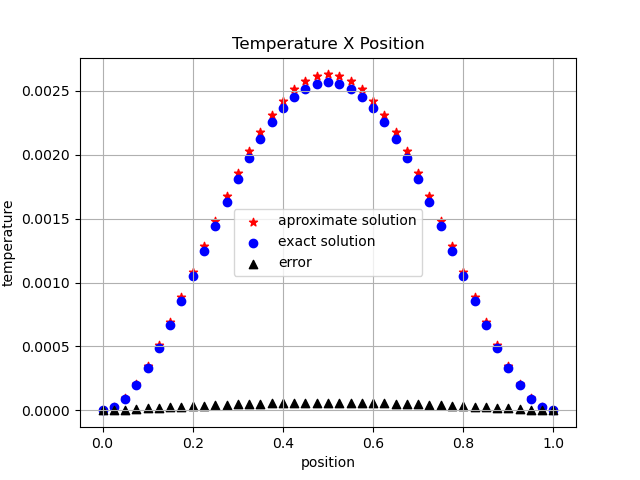
\includegraphics[scale=0.33]{graphs/a_n_40_lambda_0.25/n_40_t_0.5_lambda_0.25.png}}
	\subfigure [$t=1.0s$] {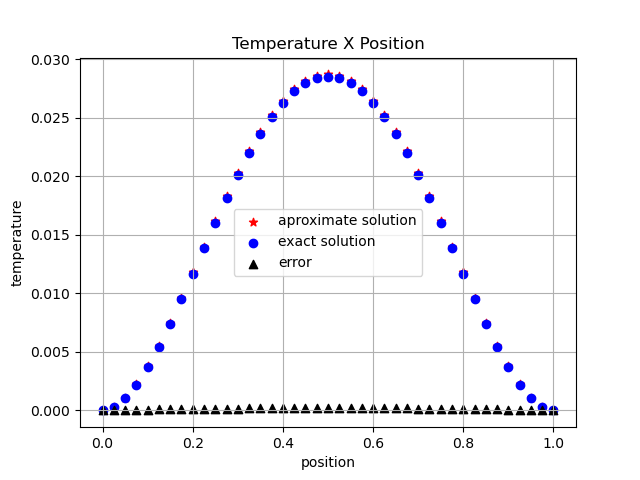
\includegraphics[scale=0.33]{graphs/a_n_40_lambda_0.25/n_40_t_1.0_lambda_0.25.png}}
	\caption{\textit{$N = 40$, $\lambda$ = 0.25}}
\end{figure} 

% Lambda igual a 0.25 e N igual a 80
\begin{figure}[H]
	\centering
	\subfigure [$t=0.1s$] {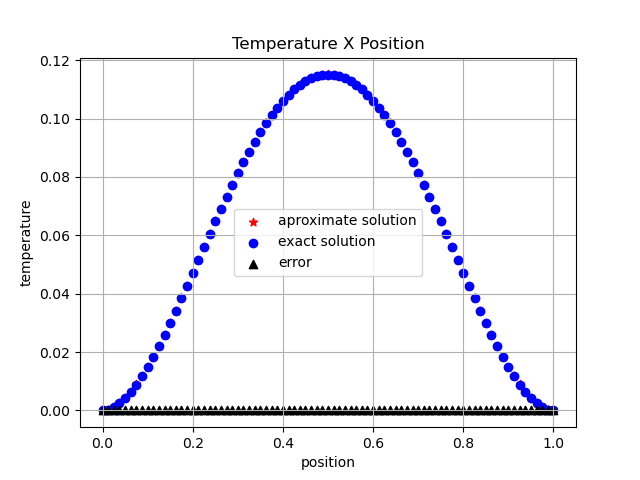
\includegraphics[scale=0.33]{graphs/a_n_80_lambda_0.25/n_80_t_0.1_lambda_0.25.png}}
	\subfigure [$t=0.5s$] {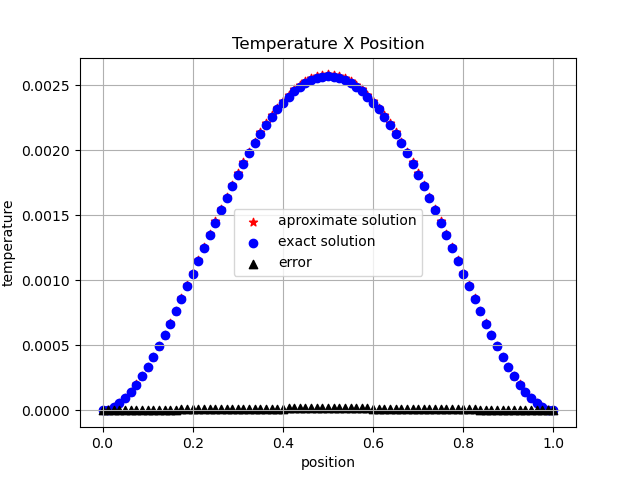
\includegraphics[scale=0.33]{graphs/a_n_80_lambda_0.25/n_80_t_0.5_lambda_0.25.png}}
	\subfigure [$t=1.0s$] {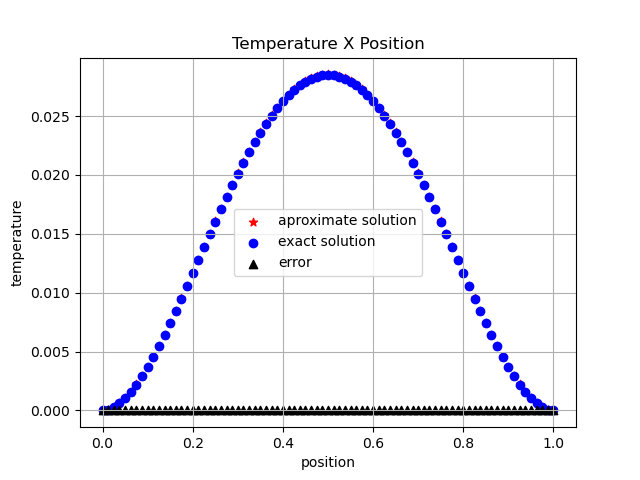
\includegraphics[scale=0.33]{graphs/a_n_80_lambda_0.25/n_80_t_1.0_lambda_0.25.png}}
	\caption{\textit{$N = 80$, $\lambda$ = 0.25}}
\end{figure} 

% Lambda igual a 0.25 e N igual a 160
\begin{figure}[H]
	\centering
	\subfigure [$t=0.1s$] {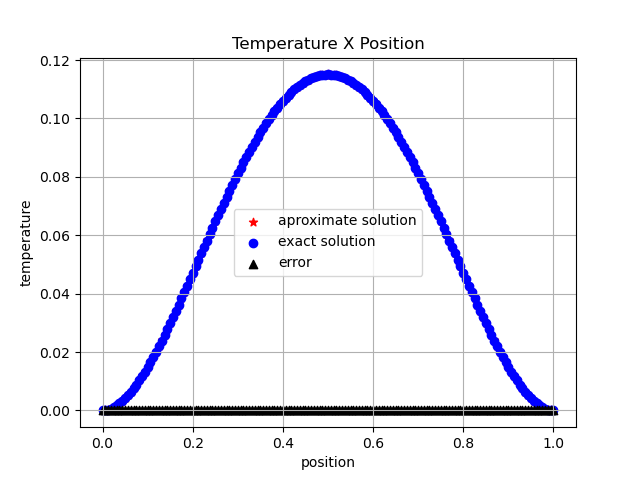
\includegraphics[scale=0.33]{graphs/a_n_160_lambda_0.25/n_160_t_0.1_lambda_0.25.png}}
	\subfigure [$t=0.5s$] {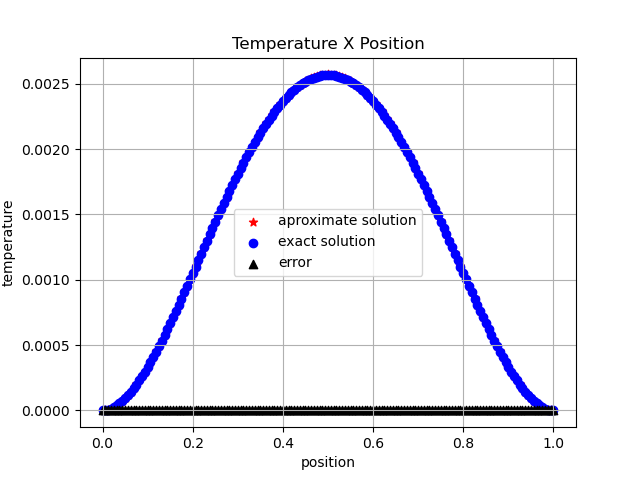
\includegraphics[scale=0.33]{graphs/a_n_160_lambda_0.25/n_160_t_0.5_lambda_0.25.png}}
	\subfigure [$t=1.0s$] {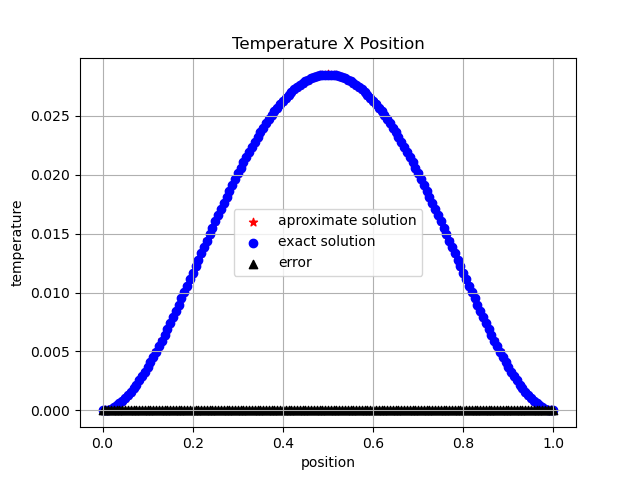
\includegraphics[scale=0.33]{graphs/a_n_160_lambda_0.25/n_160_t_1.0_lambda_0.25.png}}
	\caption{\textit{$N = 160$, $\lambda$ = 0.25}}
\end{figure}

% Lambda igual a 0.25 e N igual a 320
\begin{figure}[H]
	\centering
	\subfigure [$t=0.1s$] {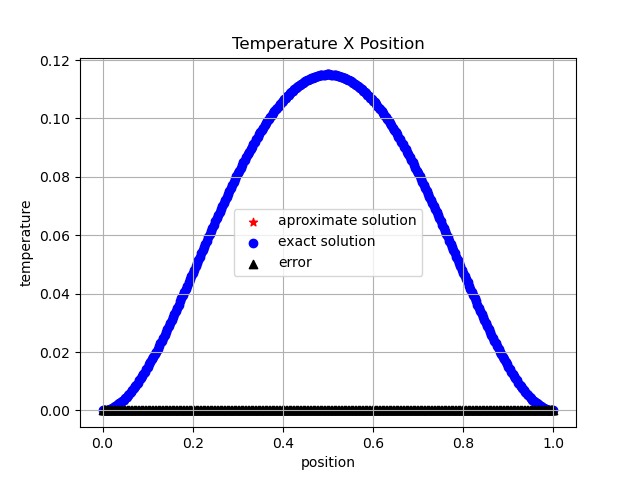
\includegraphics[scale=0.33]{graphs/a_n_320_lambda_0.25/n_320_t_0.1_lambda_0.25.png}}
	\subfigure [$t=0.5s$] {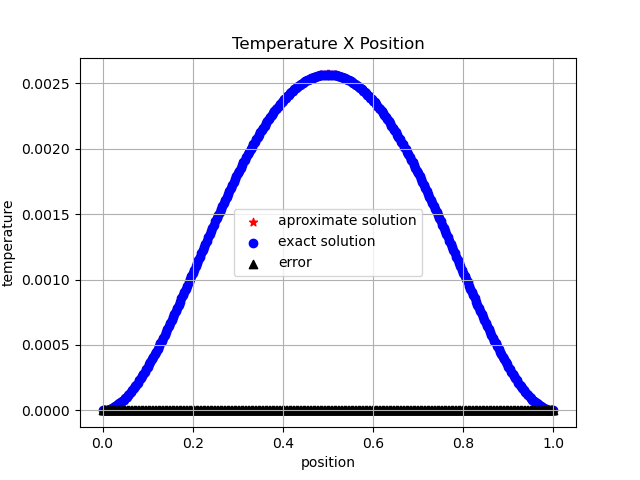
\includegraphics[scale=0.33]{graphs/a_n_320_lambda_0.25/n_320_t_0.5_lambda_0.25.png}}
	\subfigure [$t=1.0s$] {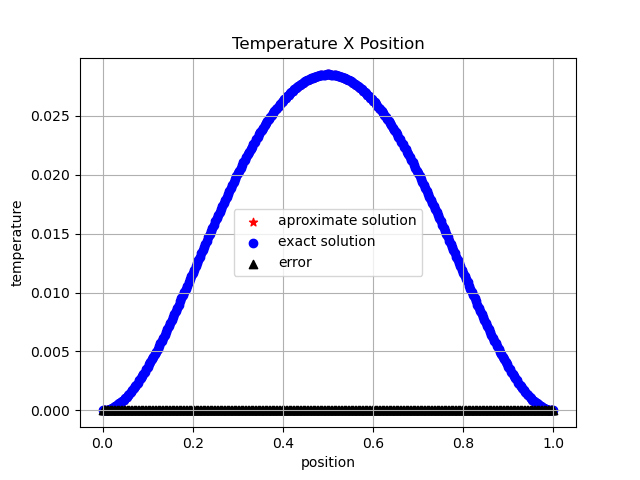
\includegraphics[scale=0.33]{graphs/a_n_320_lambda_0.25/n_320_t_1.0_lambda_0.25.png}}
	\caption{\textit{$N = 320$, $\lambda$ = 0.25}}
\end{figure}

% Lambda igual a 0.25 e N igual a 640
\begin{figure}[H]
	\centering
	\subfigure [$t=0.1s$] {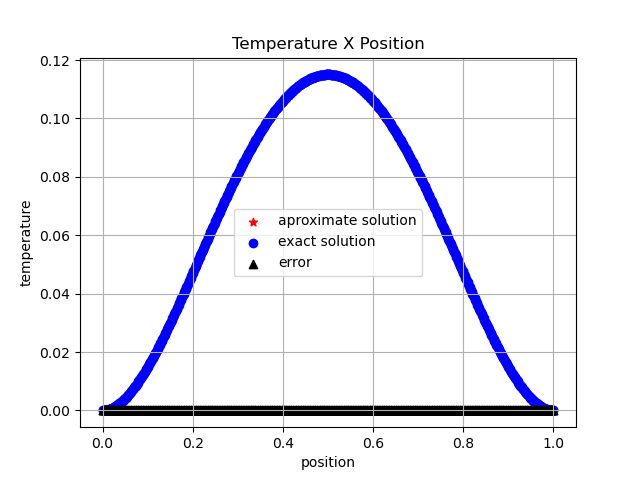
\includegraphics[scale=0.33]{graphs/a_n_640_lambda_0.25/n_640_t_0.1_lambda_0.25.png}}
	\subfigure [$t=0.5s$] {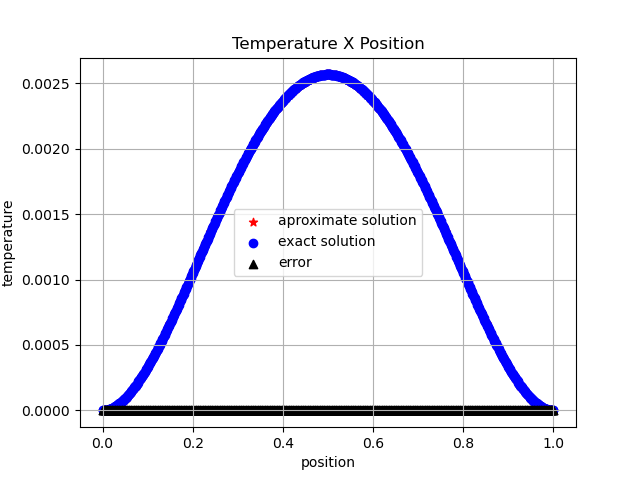
\includegraphics[scale=0.33]{graphs/a_n_640_lambda_0.25/n_640_t_0.5_lambda_0.25.png}}
	\subfigure [$t=1.0s$] {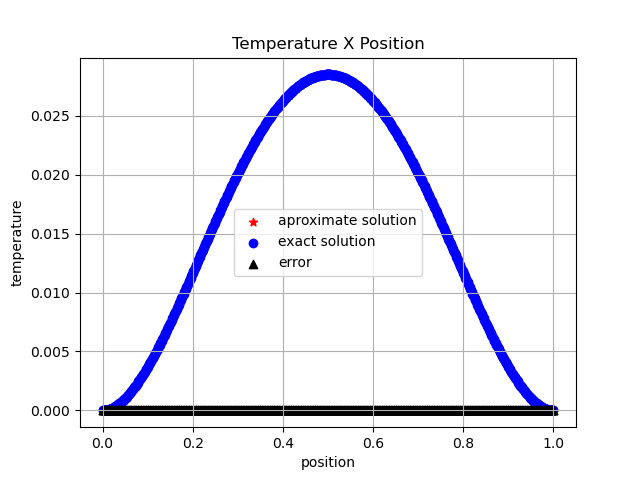
\includegraphics[scale=0.33]{graphs/a_n_640_lambda_0.25/n_640_t_1.0_lambda_0.25.png}}
	\caption{\textit{$N = 640$, $\lambda$ = 0.25}}
\end{figure}

% Lambda igual a 0.5 e N igual a 10
\begin{figure}[H]
	\centering
	\subfigure [$t=0.1s$] {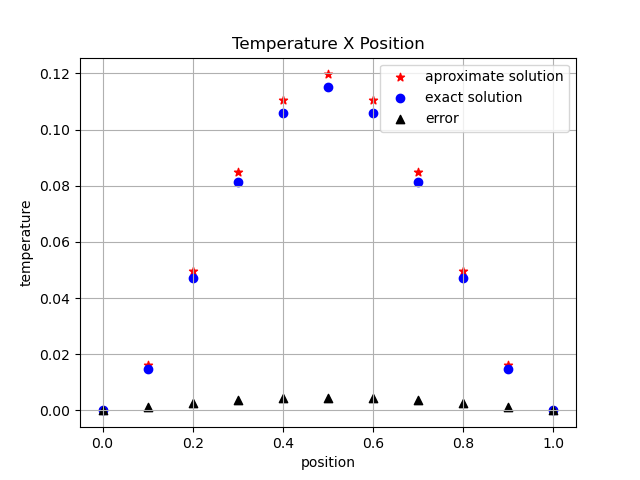
\includegraphics[scale=0.33]{graphs/a_n_10_lambda_0.5/n_10_t_0.1_lambda_0.5.png}}
	\subfigure [$t=0.5s$] {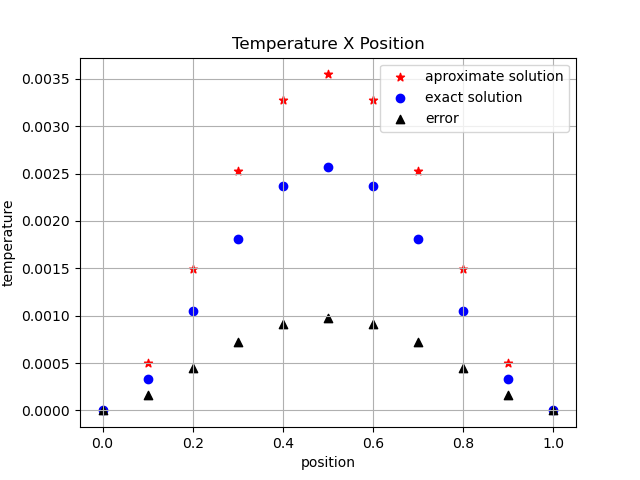
\includegraphics[scale=0.33]{graphs/a_n_10_lambda_0.5/n_10_t_0.5_lambda_0.5.png}}
	\subfigure [$t=1.0s$] {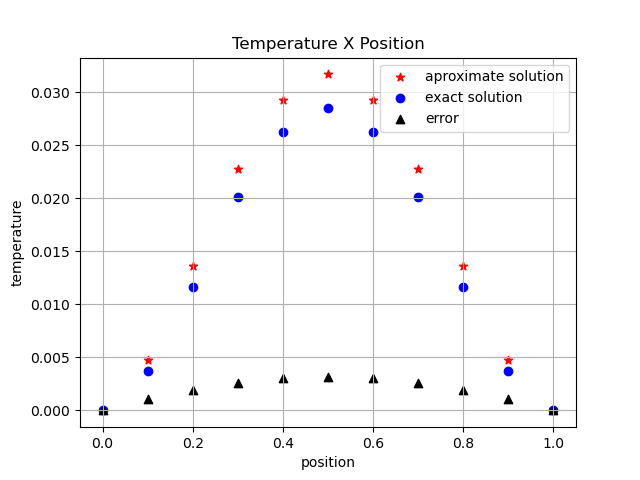
\includegraphics[scale=0.33]{graphs/a_n_10_lambda_0.5/n_10_t_1.0_lambda_0.5.png}}
	\caption{\textit{$N = 10$, $\lambda$ = 0.5}}
\end{figure}

% Lambda igual a 0.5 e N igual a 20
\begin{figure}[H]
	\centering
	\subfigure [$t=0.1s$] {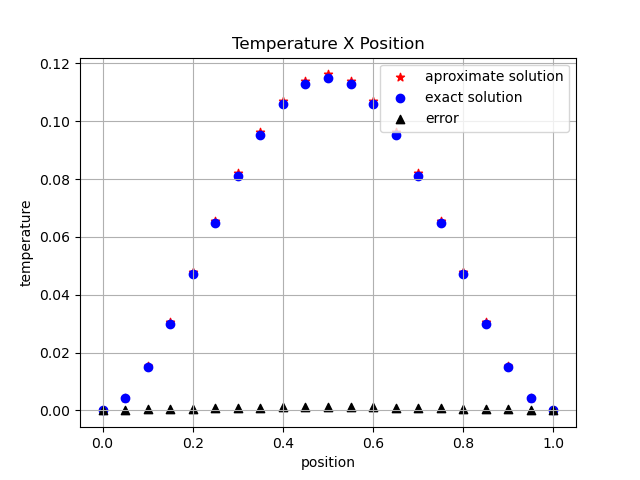
\includegraphics[scale=0.33]{graphs/a_n_20_lambda_0.5/n_20_t_0.1_lambda_0.5.png}}
	\subfigure [$t=0.5s$] {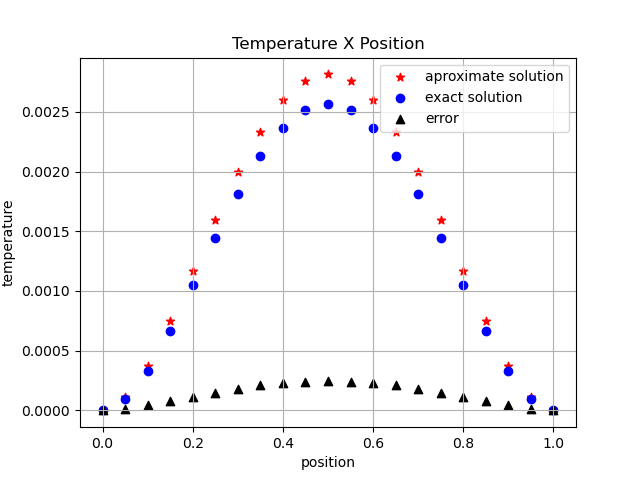
\includegraphics[scale=0.33]{graphs/a_n_20_lambda_0.5/n_20_t_0.5_lambda_0.5.png}}
	\subfigure [$t=1.0s$] {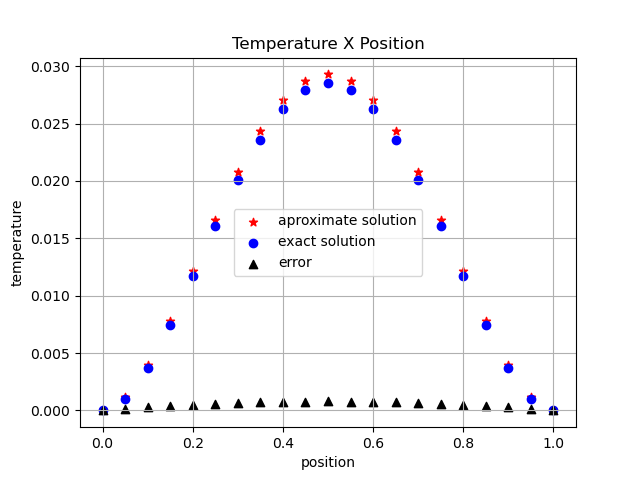
\includegraphics[scale=0.33]{graphs/a_n_20_lambda_0.5/n_20_t_1.0_lambda_0.5.png}}
	\caption{\textit{$N = 20$, $\lambda$ = 0.5}}
\end{figure}

% Lambda igual a 0.5 e N igual a 40
\begin{figure}[H]
	\centering
	\subfigure [$t=0.1s$] {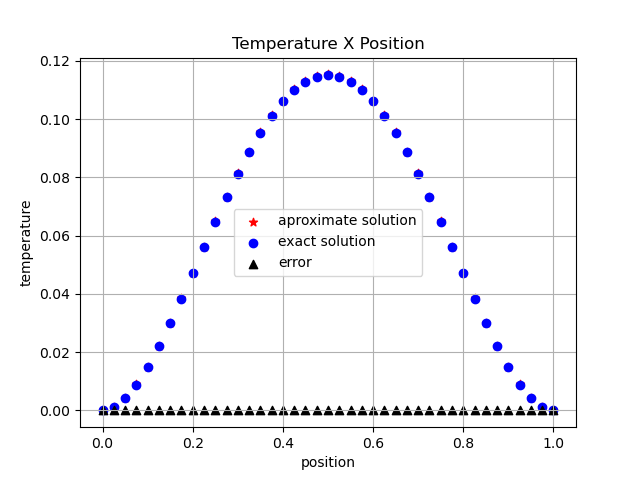
\includegraphics[scale=0.33]{graphs/a_n_40_lambda_0.5/n_40_t_0.1_lambda_0.5.png}}
	\subfigure [$t=0.5s$] {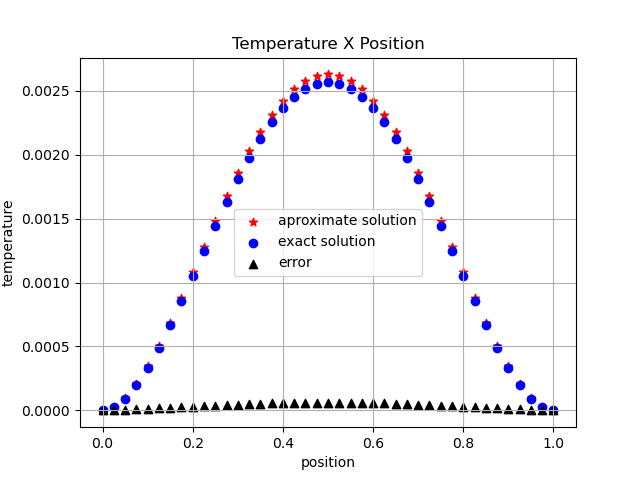
\includegraphics[scale=0.33]{graphs/a_n_40_lambda_0.5/n_40_t_0.5_lambda_0.5.png}}
	\subfigure [$t=1.0s$] {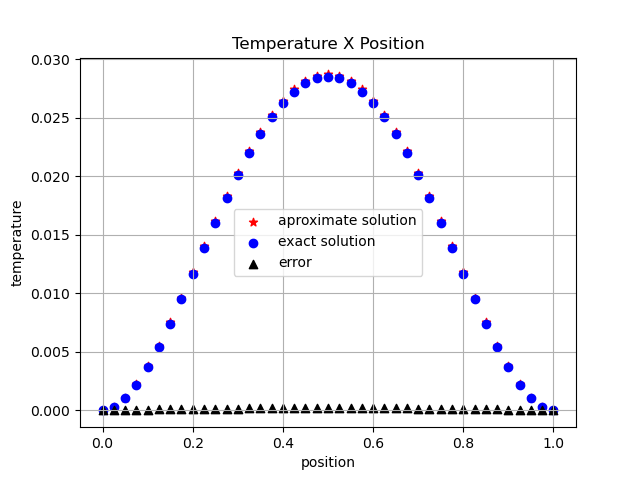
\includegraphics[scale=0.33]{graphs/a_n_40_lambda_0.5/n_40_t_1.0_lambda_0.5.png}}
	\caption{\textit{$N = 40$, $\lambda$ = 0.5}}
\end{figure}

% Lambda igual a 0.5 e N igual a 80
\begin{figure}[H]
	\centering
	\subfigure [$t=0.1s$] {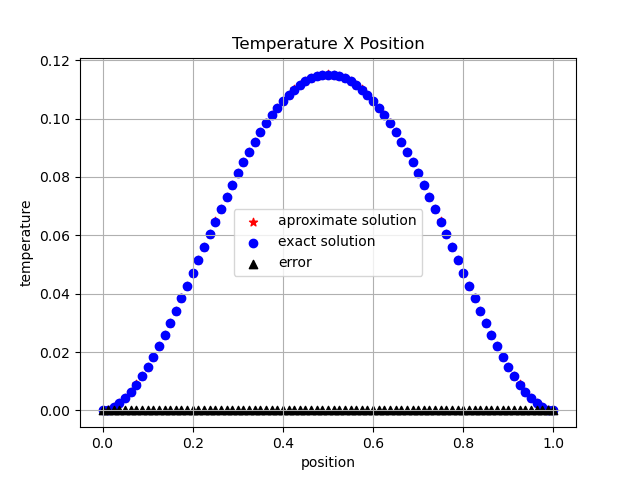
\includegraphics[scale=0.33]{graphs/a_n_80_lambda_0.5/n_80_t_0.1_lambda_0.5.png}}
	\subfigure [$t=0.5s$] {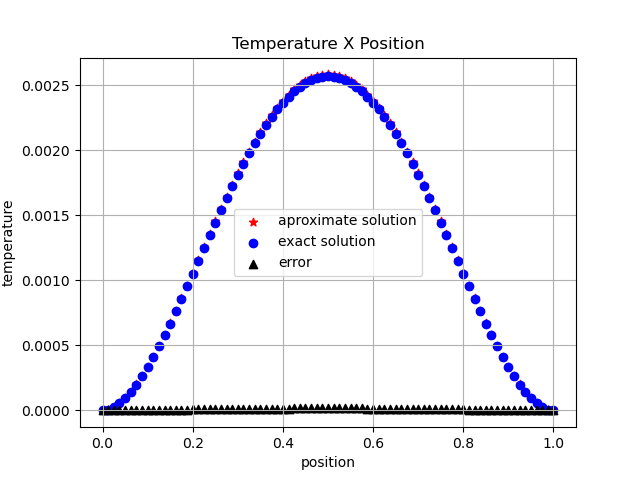
\includegraphics[scale=0.33]{graphs/a_n_80_lambda_0.5/n_80_t_0.5_lambda_0.5.png}}
	\subfigure [$t=1.0s$] {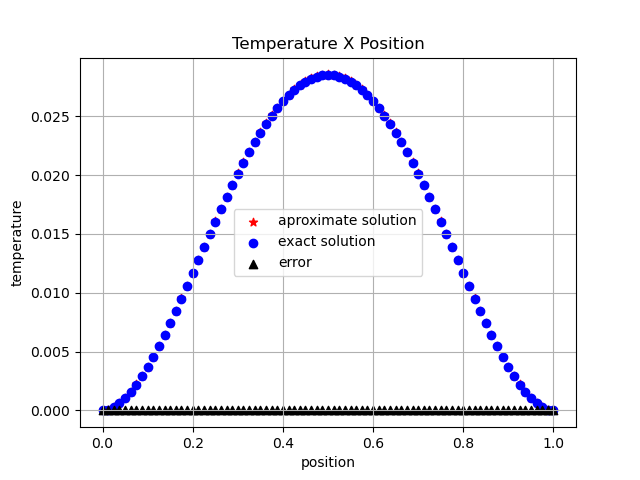
\includegraphics[scale=0.33]{graphs/a_n_80_lambda_0.5/n_80_t_1.0_lambda_0.5.png}}
	\caption{\textit{$N = 80$, $\lambda$ = 0.5}}
\end{figure}

% Lambda igual a 0.5 e N igual a 160
\begin{figure}[H]
	\centering
	\subfigure [$t=0.1s$] {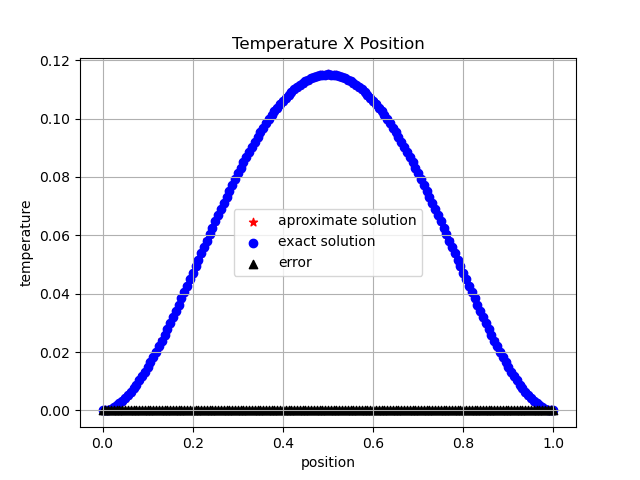
\includegraphics[scale=0.33]{graphs/a_n_160_lambda_0.5/n_160_t_0.1_lambda_0.5.png}}
	\subfigure [$t=0.5s$] {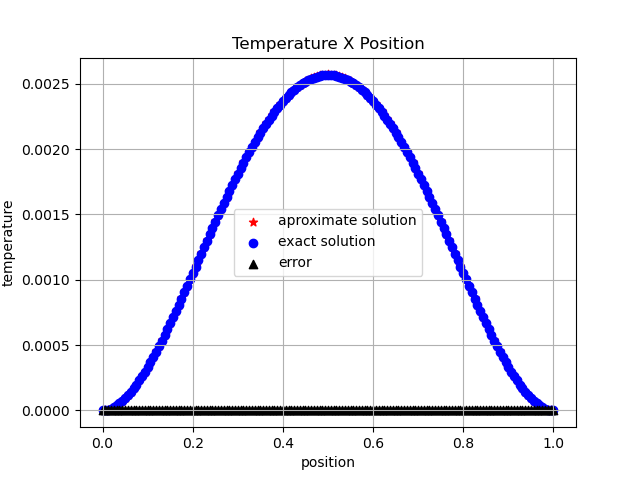
\includegraphics[scale=0.33]{graphs/a_n_160_lambda_0.5/n_160_t_0.5_lambda_0.5.png}}
	\subfigure [$t=1.0s$] {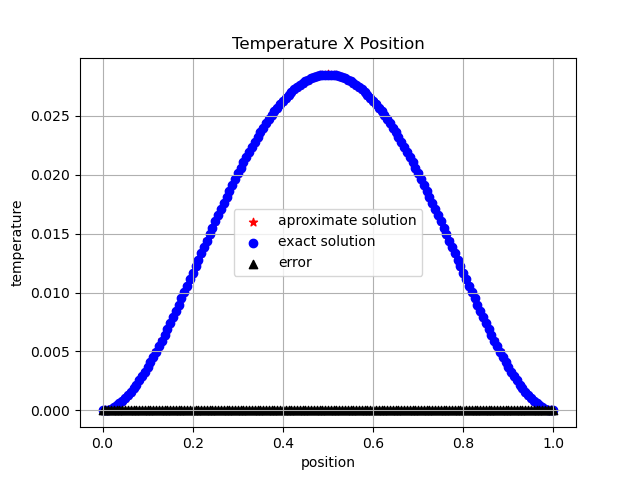
\includegraphics[scale=0.33]{graphs/a_n_160_lambda_0.5/n_160_t_1.0_lambda_0.5.png}}
	\caption{\textit{$N = 160$, $\lambda$ = 0.5}}
\end{figure}

% Lambda igual a 0.5 e N igual a 320
\begin{figure}[H]
	\centering
	\subfigure [$t=0.1s$] {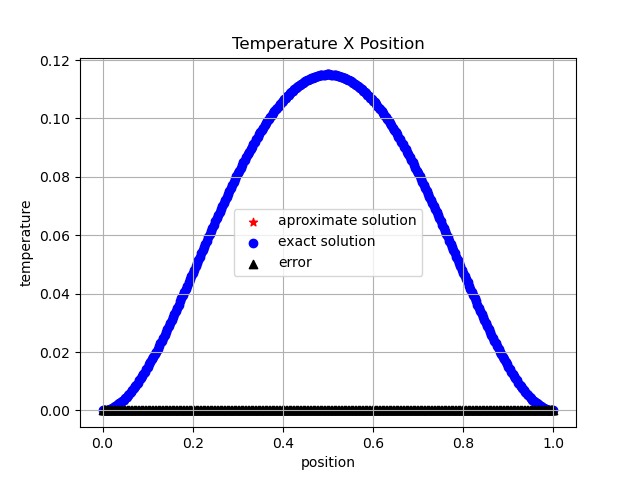
\includegraphics[scale=0.33]{graphs/a_n_320_lambda_0.5/n_320_t_0.1_lambda_0.5.png}}
	\subfigure [$t=0.5s$] {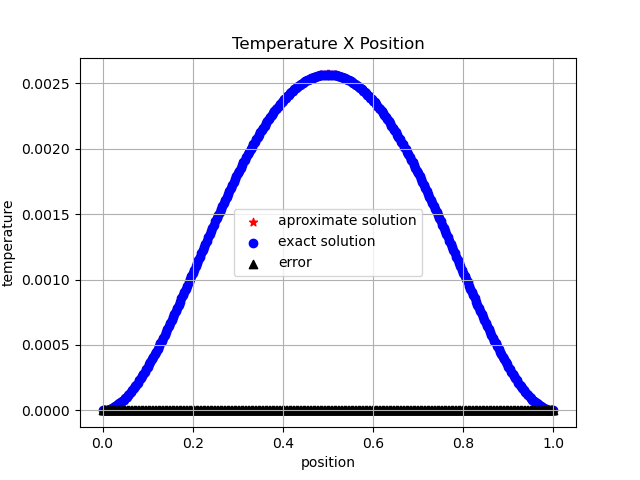
\includegraphics[scale=0.33]{graphs/a_n_320_lambda_0.5/n_320_t_0.5_lambda_0.5.png}}
	\subfigure [$t=1.0s$] {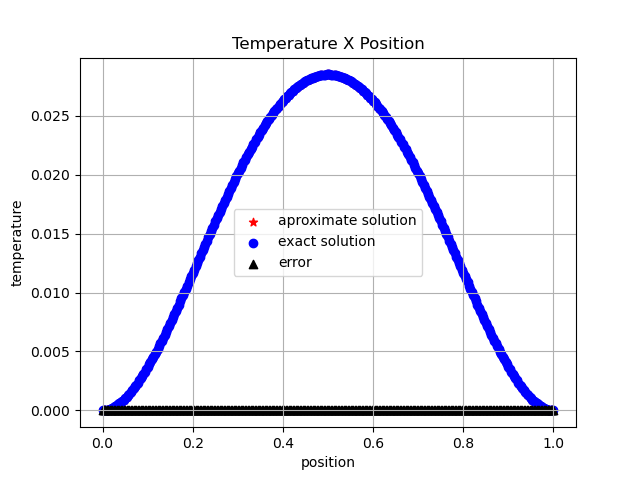
\includegraphics[scale=0.33]{graphs/a_n_320_lambda_0.5/n_320_t_1.0_lambda_0.5.png}}
	\caption{\textit{$N = 320$, $\lambda$ = 0.5}}
\end{figure}

% Lambda igual a 0.5 e N igual a 640
\begin{figure}[H]
	\centering
	\subfigure [$t=0.1s$] {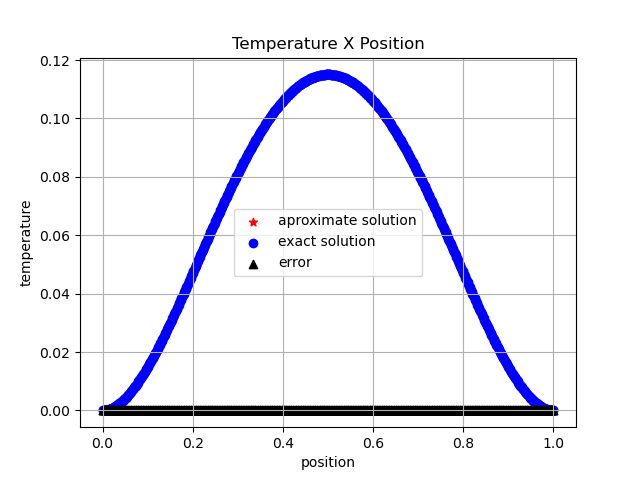
\includegraphics[scale=0.33]{graphs/a_n_640_lambda_0.5/n_640_t_0.1_lambda_0.5.png}}
	\subfigure [$t=0.5s$] {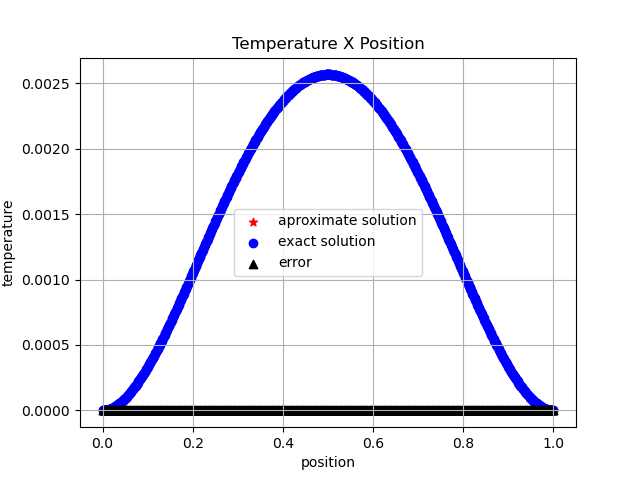
\includegraphics[scale=0.33]{graphs/a_n_640_lambda_0.5/n_640_t_0.5_lambda_0.5.png}}
	\subfigure [$t=1.0s$] {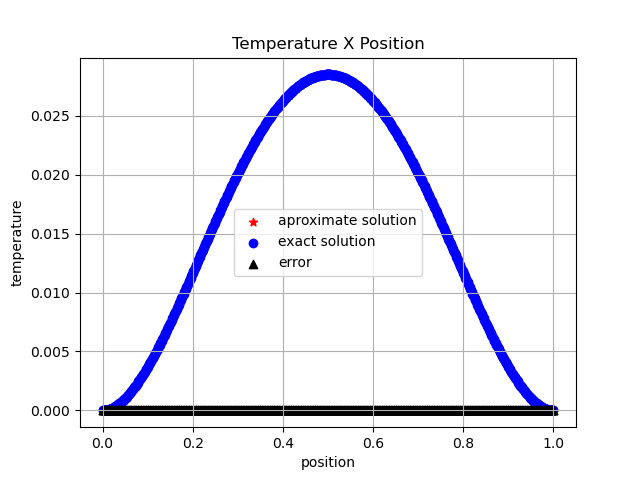
\includegraphics[scale=0.33]{graphs/a_n_640_lambda_0.5/n_640_t_1.0_lambda_0.5.png}}
	\caption{\textit{$N = 640$, $\lambda$ = 0.5}}
\end{figure}

% Lambda igual a 0.51 e N igual a 10
\begin{figure}[H]
    \centering
    \subfigure [$t=0.1s$] {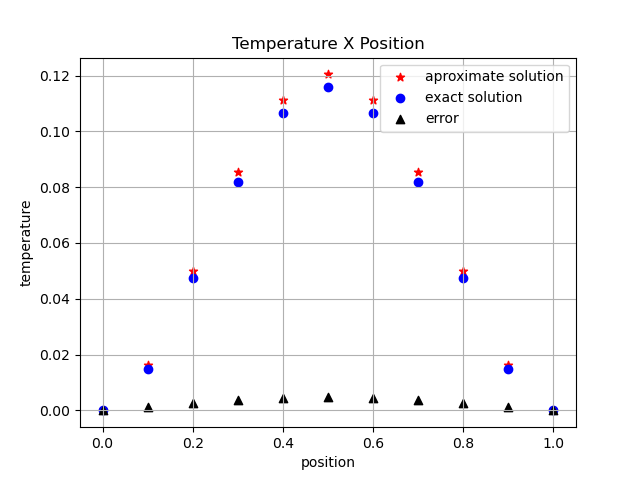
\includegraphics[scale=0.33]{graphs/a_n_10_lambda_0.51/n_10_t_0.1_lambda_0.51.png}}
	\subfigure [$t=0.5s$] {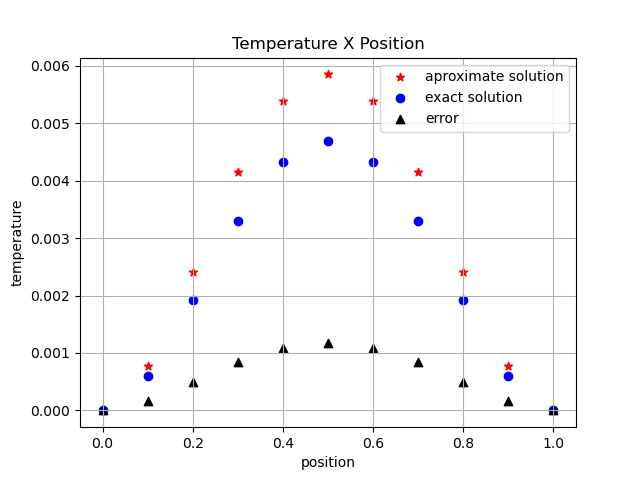
\includegraphics[scale=0.33]{graphs/a_n_10_lambda_0.51/n_10_t_0.5_lambda_0.51.png}}
	\subfigure [$t=1.0s$] {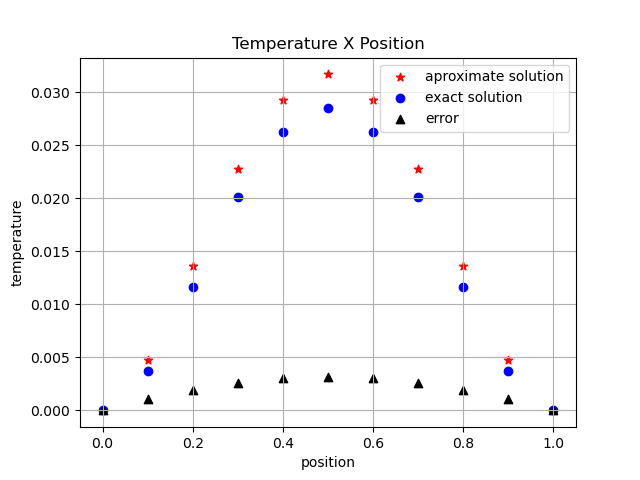
\includegraphics[scale=0.33]{graphs/a_n_10_lambda_0.51/n_10_t_1.0_lambda_0.51.png}}
    \caption{\textit{$N = 10$, $\lambda$ = 0.51}}
    
\end{figure}

% Lambda igual a 0.51 e N igual a 20
\begin{figure}[H]
    \centering
    \subfigure [$t=0.1s$] {\includegraphics[scale=0.33]{graphs/a_n_20_lambda_0.51/n_20_t_0.1_lambda_0.51.png}}
	\subfigure [$t=0.5s$] {\includegraphics[scale=0.33]{graphs/a_n_20_lambda_0.51/n_20_t_0.5_lambda_0.51.png}}
	\subfigure [$t=1.0s$] {\includegraphics[scale=0.33]{graphs/a_n_20_lambda_0.51/n_20_t_1.0_lambda_0.51.png}}
    \caption{\textit{$N = 20$, $\lambda$ = 0.51}}
    %\label{fig:my_label}
\end{figure}

% Lambda igual a 0.51 e N igual a 40
\begin{figure}[H]
    \centering
    \subfigure [$t=0.1s$] {\includegraphics[scale=0.33]{graphs/a_n_40_lambda_0.51/n_40_t_0.1_lambda_0.51.png}}
	\subfigure [$t=0.5s$] {\includegraphics[scale=0.33]{graphs/a_n_40_lambda_0.51/n_40_t_0.5_lambda_0.51.png}}
	\subfigure [$t=1.0s$] {\includegraphics[scale=0.33]{graphs/a_n_40_lambda_0.51/n_40_t_1.0_lambda_0.51.png}}
    \caption{\textit{$N = 40$, $\lambda$ = 0.51}}
    %\label{fig:my_label}
\end{figure}

% Lambda igual a 0.51 e N igual a 80
\begin{figure}[H]
    \centering
    \subfigure [$t=0.1s$] {\includegraphics[scale=0.33]{graphs/a_n_80_lambda_0.51/n_80_t_0.1_lambda_0.51.png}}
	\subfigure [$t=0.5s$] {\includegraphics[scale=0.33]{graphs/a_n_80_lambda_0.51/n_80_t_0.5_lambda_0.51.png}}
	\subfigure [$t=1.0s$] {\includegraphics[scale=0.33]{graphs/a_n_80_lambda_0.51/n_80_t_1.0_lambda_0.51.png}}
    \caption{\textit{$N = 80$, $\lambda$ = 0.51}}
    %\label{fig:my_label}
\end{figure}

% Lambda igual a 0.51 e N igual a 160
\begin{figure}[H]
    \centering
    \subfigure [$t=0.1s$] {\includegraphics[scale=0.33]{graphs/a_n_160_lambda_0.51/n_160_t_0.1_lambda_0.51.png}}
	\subfigure [$t=0.5s$] {\includegraphics[scale=0.33]{graphs/a_n_160_lambda_0.51/n_160_t_0.5_lambda_0.51.png}}
	\subfigure [$t=1.0s$] {\includegraphics[scale=0.33]{graphs/a_n_160_lambda_0.51/n_160_t_1.0_lambda_0.51.png}}
    \caption{\textit{$N = 160$, $\lambda$ = 0.51}}
    %\label{fig:my_label}
\end{figure}

% Lambda igual a 0.51 e N igual a 320
\begin{figure}[H]
    \centering
    \subfigure [$t=0.1s$] {\includegraphics[scale=0.33]{graphs/a_n_320_lambda_0.51/n_320_t_0.1_lambda_0.51.png}}
	\subfigure [$t=0.5s$] {\includegraphics[scale=0.33]{graphs/a_n_320_lambda_0.51/n_320_t_0.5_lambda_0.51.png}}
	\subfigure [$t=1.0s$] {\includegraphics[scale=0.33]{graphs/a_n_320_lambda_0.51/n_320_t_1.0_lambda_0.51.png}}
    \caption{\textit{$N = 320$, $\lambda$ = 0.51}}
\end{figure}

% Lambda igual a 0.51 e N igual a 640
\begin{figure}[H]
    \centering
    \subfigure [$t=0.1s$] {\includegraphics[scale=0.33]{graphs/a_n_640_lambda_0.51/n_640_t_0.1_lambda_0.51.png}}
	\subfigure [$t=0.5s$] {\includegraphics[scale=0.33]{graphs/a_n_640_lambda_0.51/n_640_t_0.5_lambda_0.51.png}}
	\subfigure [$t=1.0s$] {\includegraphics[scale=0.33]{graphs/a_n_640_lambda_0.51/n_640_t_1.0_lambda_0.51.png}}
    \caption{\textit{$N = 640$, $\lambda$ = 0.51}}
\end{figure}

É válido destacar que, apesar dos gráficos parecem estáticos conforme $t$ avança, é possível perceber a mudança nos valores da temperatura (eixo das ordenadas) indicando a evolução temporal.

Conforme já era esperado, as iterações com $\lambda = 0.25$ e $\lambda = 0.50$ resultaram em erros pequenos. Já para $\lambda = 0.51$, há um comportamento instável do erro e em alguns casos este cresce extraordinariamente, inclusive gerando complicações para a linguagem de programação utilizada a partir de $N=160$, onde os gráficos se tornam degenerados. Acontece que o Python não reconhece valores extremamente grandes. 

A tabela 2 apresenta resultados das normas dos erros em algumas das simulações.

% Colocar tabela com erros para cada simulação, com T=1, e diferentes resoluções de lambda
\begin{table}[!h]
    \centering
    \begin{tabular}{|c|c|c|c|}
    \hline                               % para uma linha horizontal
    N & Erro ($\lambda = 0.25$) & Erro ($\lambda = 0.50$) & Erro ($\lambda = 0.51$) \\
    \hline
    10  &  3.045e-03 & 3.164e-03 & 3.168e-03 \\
    20  &  7.578e-04 & 7.842e-04 & 7.539e+01 \\
    40  &  1.892e-04 & 1.956e-04 & 1.288e+40 \\
    80  &  4.729e-05 & 4.888e-05 & 2.650e+198 \\
    160 &  1.182e-05 & 1.222e-05 & $nan$ \\
    320 &  2.995e-06 & 3.055e-06 & $nan$ \\
    640 &  7.388e-07 & 7.637e-07 & $nan$ \\
    \hline
    \end{tabular}
    \caption{Norma do erro obtido em t = 1 para o teste $a$ com o método de Euler explícito.}
    %\label{tab:my_label}
\end{table}

Podemos definir o número de passos como sendo o número de vezes em que o programa sobrescreve o vetor $u_{new}$ no vetor $u_{old}$ ou então como o próprio número $M$. Sendo assim, utilizando $T=1$, podemos verificar que para integrações feitas com $N=640$, o número de passos do programa é igual a $\frac{640^2}{\lambda}$. Logo, para $\lambda = 0.5$ temos $M$ = 819200 e para $\lambda = 0.25$ temos $M$ = 1638400. 

Caso dobrássemos o valor de $N$, teríamos um número de passos 4 vezes maior do que quando $N=640$, o que mostra uma certa ineficiência do método utilizado ao se tentar refinar a malha. A segunda tarefa deste exercício discutirá alguns exemplos de métodos alternativos ao que foi utilizado para a primeira tarefa. 

É válido notar que uma simulação com $\lambda = 0.25$ faz o mesmo número de passos que uma simulação com $\lambda = 0.50$ mas com o dobro de N.

\subsubsection{Item (b)}

Dada a solução exata $u(t,x)=e^{t-x}cos(5tx)$ podemos determinar facilmente $u_0(x)$, $g_1(t)$ e $g_2(t)$ utilizando as condições de contorno (2), (3) e (4):

$$u_0(x)=u(0,x)=e^{-x}$$

$$g_1(t)=u(t,0)=e^{t}$$

$$g_2(t)=u(t,1)=e^{t-1}cos(5t)$$

Para determinar a fonte $f(t,x)$ o processo é análogo, utilizando (1), porém teremos que calcular algumas derivadas parciais:

$$f(t,x)=u_t(t,x)-u_{xx}(t,x)=$$ $$=e^{t-x}(cos(5tx)-5xsin(5tx))-(e^{t-x}((1-25t^2)cos(5tx)+10tsin(5tx)))=$$
$$=e^{t-x}(-5xsin(5tx)-10tsin(5tx)+25t^{2}cos(5tx))$$

\textbf{Vamos denotar essas condições por "teste b"}.

Com as condições iniciais e a fonte determinadas, podemos então repetir os procedimentos realizados para o teste $a$. Sendo assim, vamos à apresentação dos gráficos.

% Lambda igual a 0.25 e N igual a 10
\begin{figure}[H]
	\centering
    \subfigure [$t=0.1s$] {\includegraphics[scale=0.33]{graphs/b_n_10_lambda_0.25/n_10_t_0.1_lambda_0.25.png}}
	\subfigure [$t=0.5s$] {\includegraphics[scale=0.33]{graphs/b_n_10_lambda_0.25/n_10_t_0.5_lambda_0.25.png}}
	\subfigure [$t=1.0s$] {\includegraphics[scale=0.33]{graphs/b_n_10_lambda_0.25/n_10_t_1.0_lambda_0.25.png}}
	\caption{\textit{$N = 10$, $\lambda$ = 0.25}}
\end{figure}  

% Lambda igual a 0.25 e N igual a 20
\begin{figure}[H]
	\centering
    \subfigure [$t=0.1s$] {\includegraphics[scale=0.33]{graphs/b_n_20_lambda_0.25/n_20_t_0.1_lambda_0.25.png}}
	\subfigure [$t=0.5s$] {\includegraphics[scale=0.33]{graphs/b_n_20_lambda_0.25/n_20_t_0.5_lambda_0.25.png}}
	\subfigure [$t=1.0s$] {\includegraphics[scale=0.33]{graphs/b_n_20_lambda_0.25/n_20_t_1.0_lambda_0.25.png}}
	\caption{\textit{$N = 20$, $\lambda$ = 0.25}}
\end{figure}  

% Lambda igual a 0.25 e N igual a 40
\begin{figure}[H]
	\centering
	\subfigure [$t=0.1s$] {\includegraphics[scale=0.33]{graphs/b_n_40_lambda_0.25/n_40_t_0.1_lambda_0.25.png}}
	\subfigure [$t=0.5s$] {\includegraphics[scale=0.33]{graphs/b_n_40_lambda_0.25/n_40_t_0.5_lambda_0.25.png}}
	\subfigure [$t=1.0s$] {\includegraphics[scale=0.33]{graphs/b_n_40_lambda_0.25/n_40_t_1.0_lambda_0.25.png}}
	\caption{\textit{$N = 40$, $\lambda$ = 0.25}}
\end{figure} 

% Lambda igual a 0.25 e N igual a 80
\begin{figure}[H]
	\centering
	\subfigure [$t=0.1s$] {\includegraphics[scale=0.33]{graphs/b_n_80_lambda_0.25/n_80_t_0.1_lambda_0.25.png}}
	\subfigure [$t=0.5s$] {\includegraphics[scale=0.33]{graphs/b_n_80_lambda_0.25/n_80_t_0.5_lambda_0.25.png}}
	\subfigure [$t=1.0s$] {\includegraphics[scale=0.33]{graphs/b_n_80_lambda_0.25/n_80_t_1.0_lambda_0.25.png}}
	\caption{\textit{$N = 80$, $\lambda$ = 0.25}}
\end{figure} 

% Lambda igual a 0.25 e N igual a 160
\begin{figure}[H]
	\centering
	\subfigure [$t=0.1s$] {\includegraphics[scale=0.33]{graphs/b_n_160_lambda_0.25/n_160_t_0.1_lambda_0.25.png}}
	\subfigure [$t=0.5s$] {\includegraphics[scale=0.33]{graphs/b_n_160_lambda_0.25/n_160_t_0.5_lambda_0.25.png}}
	\subfigure [$t=1.0s$] {\includegraphics[scale=0.33]{graphs/b_n_160_lambda_0.25/n_160_t_1.0_lambda_0.25.png}}
	\caption{\textit{$N = 160$, $\lambda$ = 0.25}}
\end{figure}

% Lambda igual a 0.25 e N igual a 320
\begin{figure}[H]
	\centering
	\subfigure [$t=0.1s$] {\includegraphics[scale=0.33]{graphs/b_n_320_lambda_0.25/n_320_t_0.1_lambda_0.25.png}}
	\subfigure [$t=0.5s$] {\includegraphics[scale=0.33]{graphs/b_n_320_lambda_0.25/n_320_t_0.5_lambda_0.25.png}}
	\subfigure [$t=1.0s$] {\includegraphics[scale=0.33]{graphs/b_n_320_lambda_0.25/n_320_t_1.0_lambda_0.25.png}}
	\caption{\textit{$N = 320$, $\lambda$ = 0.25}}
\end{figure}

% Lambda igual a 0.25 e N igual a 640
\begin{figure}[H]
	\centering
	\subfigure [$t=0.1s$] {\includegraphics[scale=0.33]{graphs/b_n_640_lambda_0.25/n_640_t_0.1_lambda_0.25.png}}
	\subfigure [$t=0.5s$] {\includegraphics[scale=0.33]{graphs/b_n_640_lambda_0.25/n_640_t_0.5_lambda_0.25.png}}
	\subfigure [$t=1.0s$] {\includegraphics[scale=0.33]{graphs/b_n_640_lambda_0.25/n_640_t_1.0_lambda_0.25.png}}
	\caption{\textit{$N = 640$, $\lambda$ = 0.25}}
\end{figure}

% Lambda igual a 0.5 e N igual a 10
\begin{figure}[H]
	\centering
	\subfigure [$t=0.1s$] {\includegraphics[scale=0.33]{graphs/b_n_10_lambda_0.5/n_10_t_0.1_lambda_0.5.png}}
	\subfigure [$t=0.5s$] {\includegraphics[scale=0.33]{graphs/b_n_10_lambda_0.5/n_10_t_0.5_lambda_0.5.png}}
	\subfigure [$t=1.0s$] {\includegraphics[scale=0.33]{graphs/b_n_10_lambda_0.5/n_10_t_1.0_lambda_0.5.png}}
	\caption{\textit{$N = 10$, $\lambda$ = 0.5}}
\end{figure}

% Lambda igual a 0.5 e N igual a 20
\begin{figure}[H]
	\centering
	\subfigure [$t=0.1s$] {\includegraphics[scale=0.33]{graphs/b_n_20_lambda_0.5/n_20_t_0.1_lambda_0.5.png}}
	\subfigure [$t=0.5s$] {\includegraphics[scale=0.33]{graphs/b_n_20_lambda_0.5/n_20_t_0.5_lambda_0.5.png}}
	\subfigure [$t=1.0s$] {\includegraphics[scale=0.33]{graphs/b_n_20_lambda_0.5/n_20_t_1.0_lambda_0.5.png}}
	\caption{\textit{$N = 20$, $\lambda$ = 0.5}}
\end{figure}

% Lambda igual a 0.5 e N igual a 40
\begin{figure}[H]
	\centering
	\subfigure [$t=0.1s$] {\includegraphics[scale=0.33]{graphs/b_n_40_lambda_0.5/n_40_t_0.1_lambda_0.5.png}}
	\subfigure [$t=0.5s$] {\includegraphics[scale=0.33]{graphs/b_n_40_lambda_0.5/n_40_t_0.5_lambda_0.5.png}}
	\subfigure [$t=1.0s$] {\includegraphics[scale=0.33]{graphs/b_n_40_lambda_0.5/n_40_t_1.0_lambda_0.5.png}}
	\caption{\textit{$N = 40$, $\lambda$ = 0.5}}
\end{figure}

% Lambda igual a 0.5 e N igual a 80
\begin{figure}[H]
	\centering
	\subfigure [$t=0.1s$] {\includegraphics[scale=0.33]{graphs/b_n_80_lambda_0.5/n_80_t_0.1_lambda_0.5.png}}
	\subfigure [$t=0.5s$] {\includegraphics[scale=0.33]{graphs/b_n_80_lambda_0.5/n_80_t_0.5_lambda_0.5.png}}
	\subfigure [$t=1.0s$] {\includegraphics[scale=0.33]{graphs/b_n_80_lambda_0.5/n_80_t_1.0_lambda_0.5.png}}
	\caption{\textit{$N = 80$, $\lambda$ = 0.5}}
\end{figure}

% Lambda igual a 0.5 e N igual a 160
\begin{figure}[H]
	\centering
	\subfigure [$t=0.1s$] {\includegraphics[scale=0.33]{graphs/b_n_160_lambda_0.5/n_160_t_0.1_lambda_0.5.png}}
	\subfigure [$t=0.5s$] {\includegraphics[scale=0.33]{graphs/b_n_160_lambda_0.5/n_160_t_0.5_lambda_0.5.png}}
	\subfigure [$t=1.0s$] {\includegraphics[scale=0.33]{graphs/b_n_160_lambda_0.5/n_160_t_1.0_lambda_0.5.png}}
	\caption{\textit{$N = 160$, $\lambda$ = 0.5}}
\end{figure}

% Lambda igual a 0.5 e N igual a 320
\begin{figure}[H]
	\centering
	\subfigure [$t=0.1s$] {\includegraphics[scale=0.33]{graphs/b_n_320_lambda_0.5/n_320_t_0.1_lambda_0.5.png}}
	\subfigure [$t=0.5s$] {\includegraphics[scale=0.33]{graphs/b_n_320_lambda_0.5/n_320_t_0.5_lambda_0.5.png}}
	\subfigure [$t=1.0s$] {\includegraphics[scale=0.33]{graphs/b_n_320_lambda_0.5/n_320_t_1.0_lambda_0.5.png}}
	\caption{\textit{$N = 320$, $\lambda$ = 0.5}}
\end{figure}

% Lambda igual a 0.5 e N igual a 640
\begin{figure}[H]
	\centering
	\subfigure [$t=0.1s$] {\includegraphics[scale=0.33]{graphs/b_n_640_lambda_0.5/n_640_t_0.1_lambda_0.5.png}}
	\subfigure [$t=0.5s$] {\includegraphics[scale=0.33]{graphs/b_n_640_lambda_0.5/n_640_t_0.5_lambda_0.5.png}}
	\subfigure [$t=1.0s$] {\includegraphics[scale=0.33]{graphs/b_n_640_lambda_0.5/n_640_t_1.0_lambda_0.5.png}}
	\caption{\textit{$N = 640$, $\lambda$ = 0.5}}
\end{figure}

% Lambda igual a 0.51 e N igual a 10
\begin{figure}[H]
    \centering
    \subfigure [$t=0.1s$] {\includegraphics[scale=0.33]{graphs/b_n_10_lambda_0.51/n_10_t_0.1_lambda_0.51.png}}
	\subfigure [$t=0.5s$] {\includegraphics[scale=0.33]{graphs/b_n_10_lambda_0.51/n_10_t_0.5_lambda_0.51.png}}
	\subfigure [$t=1.0s$] {\includegraphics[scale=0.33]{graphs/b_n_10_lambda_0.51/n_10_t_1.0_lambda_0.51.png}}
    \caption{\textit{$N = 10$, $\lambda$ = 0.51}}
    
\end{figure}

% Lambda igual a 0.51 e N igual a 20
\begin{figure}[H]
    \centering
    \subfigure [$t=0.1s$] {\includegraphics[scale=0.33]{graphs/b_n_20_lambda_0.51/n_20_t_0.1_lambda_0.51.png}}
	\subfigure [$t=0.5s$] {\includegraphics[scale=0.33]{graphs/b_n_20_lambda_0.51/n_20_t_0.5_lambda_0.51.png}}
	\subfigure [$t=1.0s$] {\includegraphics[scale=0.33]{graphs/b_n_20_lambda_0.51/n_20_t_1.0_lambda_0.51.png}}
    \caption{\textit{$N = 20$, $\lambda$ = 0.51}}
    %\label{fig:my_label}
\end{figure}

% Lambda igual a 0.51 e N igual a 40
\begin{figure}[H]
    \centering
    \subfigure [$t=0.1s$] {\includegraphics[scale=0.33]{graphs/b_n_40_lambda_0.51/n_40_t_0.1_lambda_0.51.png}}
	\subfigure [$t=0.5s$] {\includegraphics[scale=0.33]{graphs/b_n_40_lambda_0.51/n_40_t_0.5_lambda_0.51.png}}
	\subfigure [$t=1.0s$] {\includegraphics[scale=0.33]{graphs/b_n_40_lambda_0.51/n_40_t_1.0_lambda_0.51.png}}
    \caption{\textit{$N = 40$, $\lambda$ = 0.51}}
    %\label{fig:my_label}
\end{figure}

% Lambda igual a 0.51 e N igual a 80
\begin{figure}[H]
    \centering
    \subfigure [$t=0.1s$] {\includegraphics[scale=0.33]{graphs/b_n_80_lambda_0.51/n_80_t_0.1_lambda_0.51.png}}
	\subfigure [$t=0.5s$] {\includegraphics[scale=0.33]{graphs/b_n_80_lambda_0.51/n_80_t_0.5_lambda_0.51.png}}
	\subfigure [$t=1.0s$] {\includegraphics[scale=0.33]{graphs/b_n_80_lambda_0.51/n_80_t_1.0_lambda_0.51.png}}
    \caption{\textit{$N = 80$, $\lambda$ = 0.51}}
    %\label{fig:my_label}
\end{figure}

% Lambda igual a 0.51 e N igual a 160
\begin{figure}[H]
    \centering
    \subfigure [$t=0.1s$] {\includegraphics[scale=0.33]{graphs/b_n_160_lambda_0.51/n_160_t_0.1_lambda_0.51.png}}
	\subfigure [$t=0.5s$] {\includegraphics[scale=0.33]{graphs/b_n_160_lambda_0.51/n_160_t_0.5_lambda_0.51.png}}
	\subfigure [$t=1.0s$] {\includegraphics[scale=0.33]{graphs/b_n_160_lambda_0.51/n_160_t_1.0_lambda_0.51.png}}
    \caption{\textit{$N = 160$, $\lambda$ = 0.51}}
    %\label{fig:my_label}
\end{figure}

% Lambda igual a 0.51 e N igual a 320
\begin{figure}[H]
    \centering
    \subfigure [$t=0.1s$] {\includegraphics[scale=0.33]{graphs/b_n_320_lambda_0.51/n_320_t_0.1_lambda_0.51.png}}
	\subfigure [$t=0.5s$] {\includegraphics[scale=0.33]{graphs/b_n_320_lambda_0.51/n_320_t_0.5_lambda_0.51.png}}
	\subfigure [$t=1.0s$] {\includegraphics[scale=0.33]{graphs/b_n_320_lambda_0.51/n_320_t_1.0_lambda_0.51.png}}
    \caption{\textit{$N = 320$, $\lambda$ = 0.51}}
\end{figure}

% Lambda igual a 0.51 e N igual a 640
\begin{figure}[H]
    \centering
    \subfigure [$t=0.1s$] {\includegraphics[scale=0.33]{graphs/b_n_640_lambda_0.51/n_640_t_0.1_lambda_0.51.png}}
	\subfigure [$t=0.5s$] {\includegraphics[scale=0.33]{graphs/b_n_640_lambda_0.51/n_640_t_0.5_lambda_0.51.png}}
	\subfigure [$t=1.0s$] {\includegraphics[scale=0.33]{graphs/b_n_640_lambda_0.51/n_640_t_1.0_lambda_0.51.png}}
    \caption{\textit{$N = 640$, $\lambda$ = 0.51}}
\end{figure}

Também podemos analisar o erro, assim como feito no item anterior: 

\begin{table}[!h]
    \centering
    \begin{tabular}{|c|c|c|c|}
    \hline                               % para uma linha horizontal
    N & Erro ($\lambda = 0.25$) & Erro ($\lambda = 0.50$) & Erro ($\lambda = 0.51$) \\
    \hline
    10  & 5.005e-02  & 5.045e-02 & 5.047e-02   \\
    20  & 1.250e-02  & 1.258e-02 & 3.988e+01   \\
    40  & 3.129e-03  & 3.154e-03 & 6.798e+39  \\
    80  & 7.819e-04  & 7.882e-04 & 1.398e+198 \\
    160 & 1.955e-05  & 1.970e-04 &  $nan$ \\
    320 & 4.887e-05  & 4.926e-05 &  $nan$ \\
    640 & 1.222e-05  & 1.231e-05 &  $nan$ \\
    \hline
    \end{tabular}
    \caption{Norma do erro obtido em t = 1 para o teste $b$ com o método de Euler explícito.}
    %\label{tab:my_label}
\end{table}

Notemos que, a partir de $N=160$, com $\lambda=0.51$, os gráficos se tornam degenerados. Apesar de parecer que a solução aproximada é igual a solução exata, com erro nulo, o que ocorre na verdade é o contrário, com um erro tão grande que o Python é incapaz de reconhecer.

Conforme esperado pela teoria, a norma do erro diminui com o aumento de $N$ e aumenta com o aumento de $\lambda$. O fator de redução da norma do erro a cada vez que dobramos $N$ é $\frac{1}{4}$, valor este que é determinado ao analisar a demonstração de convergência do método e pode ser verificado na tabela 3. 

\subsubsection{Item (c)}
Nesta etapa da tarefa, tivemos que implementar uma fonte pontual localizada em um ponto $p$ do domínio e intensidade variando ao longo do tempo. A fonte foi fixada na posição $p=0.25$ e a intensidade era dada por $r(t) = 10000({1 - 2t^2})$ com a fonte $f(t, x) = r(t)g_{h}(x)$, onde $g_{h}(x)$ segue a equação abaixo:


\begin{eqnarray}
g_{h}(x) =\frac{1}{h}, \hspace{0.2cm} se \hspace{0.2cm} (p {-}\frac{h}{2}) \leq  x \leq (p + \frac{h}{2}),\hspace{0.2cm} e \hspace{0.2cm} g_{h}(x) = 0 \hspace{0.2cm} caso\hspace{0.2cm} contrario, \hspace{0.2cm} com \hspace{0.2cm} h = \Delta x
\label{eqn:ghx}
\end{eqnarray}

\textbf{Vamos denotar essas condições por "teste c"}.

As próximas imagens representam o resultado obtido. Foram seguidas as mesmas etapas dos exercícios anteriores. Neste exercício em específico não foi pedido para que calculássemos o erro, pois teríamos que determinar numericamente a solução exata, que se encontra abaixo:

% Colocar as fotos do item (c)

% Lambda igual a 0.25 e N igual a 10
\begin{figure}[H]
	\centering
    \subfigure [$t=0.1s$] {\includegraphics[scale=0.33]{graphs/c_n_10_lambda_0.25/n_10_t_0.1_lambda_0.25.png}}
	\subfigure [$t=0.5s$] {\includegraphics[scale=0.33]{graphs/c_n_10_lambda_0.25/n_10_t_0.5_lambda_0.25.png}}
	\subfigure [$t=1.0s$] {\includegraphics[scale=0.33]{graphs/c_n_10_lambda_0.25/n_10_t_1.0_lambda_0.25.png}}
	\caption{\textit{$N = 10$, $\lambda$ = 0.25}}
\end{figure}  

% Lambda igual a 0.25 e N igual a 320
\begin{figure}[H]
	\centering
	\subfigure [$t=0.1s$] {\includegraphics[scale=0.33]{graphs/c_n_320_lambda_0.25/n_320_t_0.1_lambda_0.25.png}}
	\subfigure [$t=0.5s$] {\includegraphics[scale=0.33]{graphs/c_n_320_lambda_0.25/n_320_t_0.5_lambda_0.25.png}}
	\subfigure [$t=1.0s$] {\includegraphics[scale=0.33]{graphs/c_n_320_lambda_0.25/n_320_t_1.0_lambda_0.25.png}}
	\caption{\textit{$N = 320$, $\lambda$ = 0.25}}
\end{figure}

% Lambda igual a 0.25 e N igual a 640
\begin{figure}[H]
	\centering
	\subfigure [$t=0.1s$] {\includegraphics[scale=0.33]{graphs/c_n_640_lambda_0.25/n_640_t_0.1_lambda_0.25.png}}
	\subfigure [$t=0.5s$] {\includegraphics[scale=0.33]{graphs/c_n_640_lambda_0.25/n_640_t_0.5_lambda_0.25.png}}
	\subfigure [$t=1.0s$] {\includegraphics[scale=0.33]{graphs/c_n_640_lambda_0.25/n_640_t_1.0_lambda_0.25.png}}
	\caption{\textit{$N = 640$, $\lambda$ = 0.25}}
\end{figure}

% Lambda igual a 0.5 e N igual a 10
\begin{figure}[H]
	\centering
	\subfigure [$t=0.1s$] {\includegraphics[scale=0.33]{graphs/c_n_10_lambda_0.5/n_10_t_0.1_lambda_0.50.png}}
	\subfigure [$t=0.5s$] {\includegraphics[scale=0.33]{graphs/c_n_10_lambda_0.5/n_10_t_0.5_lambda_0.50.png}}
	\subfigure [$t=1.0s$] {\includegraphics[scale=0.33]{graphs/c_n_10_lambda_0.5/n_10_t_1.0_lambda_0.50.png}}
	\caption{\textit{$N = 10$, $\lambda$ = 0.5}}
\end{figure}

% Lambda igual a 0.5 e N igual a 320
\begin{figure}[H]
	\centering
	\subfigure [$t=0.1s$] {\includegraphics[scale=0.33]{graphs/c_n_320_lambda_0.5/n_320_t_0.1_lambda_0.5.png}}
	\subfigure [$t=0.5s$] {\includegraphics[scale=0.33]{graphs/c_n_320_lambda_0.5/n_320_t_0.5_lambda_0.5.png}}
	\subfigure [$t=1.0s$] {\includegraphics[scale=0.33]{graphs/c_n_320_lambda_0.5/n_320_t_1.0_lambda_0.5.png}}
	\caption{\textit{$N = 320$, $\lambda$ = 0.5}}
\end{figure}

% Lambda igual a 0.5 e N igual a 640
\begin{figure}[H]
	\centering
	\subfigure [$t=0.1s$] {\includegraphics[scale=0.33]{graphs/c_n_640_lambda_0.5/n_640_t_0.1_lambda_0.5.png}}
	\subfigure [$t=0.2s$] {\includegraphics[scale=0.33]{graphs/c_n_640_lambda_0.5/n_640_t_0.2_lambda_0.5.png}}
	\subfigure [$t=0.3s$] {\includegraphics[scale=0.33]{graphs/c_n_640_lambda_0.5/n_640_t_0.3_lambda_0.5.png}}
	\subfigure [$t=0.4s$] {\includegraphics[scale=0.33]{graphs/c_n_640_lambda_0.5/n_640_t_0.4_lambda_0.5.png}}
	\subfigure [$t=0.5s$] {\includegraphics[scale=0.33]{graphs/c_n_640_lambda_0.5/n_640_t_0.5_lambda_0.5.png}}
	\subfigure [$t=0.6s$] {\includegraphics[scale=0.33]{graphs/c_n_640_lambda_0.5/n_640_t_0.6_lambda_0.5.png}}
	\subfigure [$t=0.7s$] {\includegraphics[scale=0.33]{graphs/c_n_640_lambda_0.5/n_640_t_0.7_lambda_0.5.png}}
	\subfigure [$t=0.8s$] {\includegraphics[scale=0.33]{graphs/c_n_640_lambda_0.5/n_640_t_0.8_lambda_0.5.png}}
	\subfigure [$t=0.9s$] {\includegraphics[scale=0.33]{graphs/c_n_640_lambda_0.5/n_640_t_0.9_lambda_0.5.png}}
	\subfigure [$t=1.0s$] {\includegraphics[scale=0.33]{graphs/c_n_640_lambda_0.5/n_640_t_1.0_lambda_0.5.png}}
	\caption{\textit{$N = 640$, $\lambda$ = 0.5}}
\end{figure}

Na figura 49, com $N=640$ e $\lambda = 0.5$, é possível observar a evolução temporal da temperatura em função da posição para os instantes de tempo de $0.1s$ até $1.0s$, sendo essa a solução exata numérica. Nos demais casos optou-se por representar somente os instantes de tempo $0.1s$, $0.5s$ e $1.0s$ para evitar a exposição de muitos gráficos. 


\subsection{Segunda tarefa}

Nesta segunda tarefa nos foi solicitado a implementação de dois métodos implícitos: \textit{Euler} e \textit{Crank-Nicolson}. Para tal, é necessário, em cada caso, resolver um sistema linear com uma matriz $A$ tridiagonal simétrica a cada passo no tempo. Para resolvermos este sistema é conveniente que a matriz $A$ seja decomposta em outras 3 matrizes do tipo:

$$
A=LDL^t
$$

Assim, fica mais simples resolvermos o sistema:

$$
LDL^{t} x = b
$$

Vale notar que, conforme descrito anteriormente nas equações (9) e (11), as matrizes $A$ e $b$ mudam de acordo com o método. 

Nos itens a seguir iremos explicar como é feita a decomposição da matriz $A$ e como o sistema linear é resolvido, bem como apresentar os resultados obtidos ao executar o programa para os 2 métodos implícitos implementados.

\subsubsection{Item (a)}

Inicialmente é preciso decompor a matriz $A$. Para isso, foi criada uma função \\ \textit{decomp(vet1, vet2)} $\rightarrow$ \textit{(vet\_d, vet\_l)} que recebe os vetores \textit{vet1} e \textit{vet2}, os quais representam a diagonal principal e a subdiagonal da matriz $A$; e retorna os vetores \textit{vet\_d} e \textit{vet\_l}, os quais representam as matrizes $D$ e $L$ respectivamente.

\begin{figure}[H]
	\centering
	\includegraphics[scale=0.5]{img/decomp.png}
	\caption{\textit{Função decomp}}
\end{figure}

Com a matriz $A$ decomposta e tendo os vetores que representam as matrizes $D$ e $L$, podemos implementar a rotina que resolve o sistema desejado. Para a implementação desta rotina recorreu-se ao livro base da disciplina \textbf{Burden \& Faires - Análise Numérica}, onde o autor descreve um pseudo-código que resolve o sistema linear. A resolução do sistema ocorre em 3 etapas:

\begin{enumerate}[i]
	
	\item Resolução do sistema $Ly=b$;
	
	\item Resolução do sistema $Dz=y$
	
	\item Resolução do sistema $L^{t}x=z$

\end{enumerate}

Foi criada, então, uma função \textit{solve\_sys} que recebe os 4 vetores que caracterizam o sistema linear e retorna o vetor solução. 

\begin{figure}[H]
	\centering
	\includegraphics[scale=0.5]{img/solve_sys.png}
	\caption{\textit{Função solve\_sys}}
\end{figure}

Tendo essas duas rotinas criadas, somos capazes de implementar os 2 métodos implícitos pedidos.

\subsubsection{Item (b)}

Para executar os testes pelos métodos de \textit{Euler} e \textit{Crank-Nicolson} com a condição $\Delta t = \Delta x$ devemos nos atentar à alguns pontos. O primeiro deles é que o usuário não mais determina o valor de $\lambda$ livremente, sendo este parâmetro determinado por:

$$
\lambda = \frac{\Delta t}{\Delta x^2} = \frac{1}{\Delta x} = N
$$

Ou, por outro lado:

$$
\lambda = \frac{\Delta t}{\Delta x^2} = \frac{1}{\Delta t} = \frac{M}{T} = N
$$

Note que a última passagem vem do fato de que $\Delta t = \Delta x$ $\Rightarrow$ $\frac{M}{T} = N$.

Portanto, em tempo de execução, o usuário só determina o parâmetro $N=\lambda$ e o parâmetro $M$ é determinado por $M=NT$. Para efeitos de testes iremos utilizar $T=1$ $\Rightarrow$ $M=N$, porém o programa foi configurado para receber qualquer valor positivo $T$.

Dito isso, vamos então à apresentação dos gráficos para o método de \textit{Euler implícito}:

% N igual a 10
\begin{figure}[H]
	\centering
	\subfigure [$t=0.1s$] {\includegraphics[scale=0.33]{graphs/Euler/a/n_10/n_10_t_0.1.png}}
	\subfigure [$t=0.5s$] {\includegraphics[scale=0.33]{graphs/Euler/a/n_10/n_10_t_0.5.png}}
	\subfigure [$t=1.0s$] {\includegraphics[scale=0.33]{graphs/Euler/a/n_10/n_10_t_1.0.png}}
	\caption{\textit{$N = 10$, teste a}}
\end{figure}

% N igual a 20
\begin{figure}[H]
	\centering
	\subfigure [$t=0.1s$] {\includegraphics[scale=0.33]{graphs/Euler/a/n_20/n_20_t_0.1.png}}
	\subfigure [$t=0.5s$] {\includegraphics[scale=0.33]{graphs/Euler/a/n_20/n_20_t_0.5.png}}
	\subfigure [$t=1.0s$] {\includegraphics[scale=0.33]{graphs/Euler/a/n_20/n_20_t_1.0.png}}
	\caption{\textit{$N = 20$, teste a}}
\end{figure}

% N igual a 40
\begin{figure}[H]
	\centering
	\subfigure [$t=0.1s$] {\includegraphics[scale=0.33]{graphs/Euler/a/n_40/n_40_t_0.1.png}}
	\subfigure [$t=0.5s$] {\includegraphics[scale=0.33]{graphs/Euler/a/n_40/n_40_t_0.5.png}}
	\subfigure [$t=1.0s$] {\includegraphics[scale=0.33]{graphs/Euler/a/n_40/n_40_t_1.0.png}}
	\caption{\textit{$N = 40$, teste a}}
\end{figure}

% N igual a 80
\begin{figure}[H]
	\centering
	\subfigure [$t=0.1s$] {\includegraphics[scale=0.33]{graphs/Euler/a/n_80/n_80_t_0.1.png}}
	\subfigure [$t=0.5s$] {\includegraphics[scale=0.33]{graphs/Euler/a/n_80/n_80_t_0.5.png}}
	\subfigure [$t=1.0s$] {\includegraphics[scale=0.33]{graphs/Euler/a/n_80/n_80_t_1.0.png}}
	\caption{\textit{$N = 80$, teste a}}
\end{figure}

% N igual a 160
\begin{figure}[H]
	\centering
	\subfigure [$t=0.1s$] {\includegraphics[scale=0.33]{graphs/Euler/a/n_160/n_160_t_0.1.png}}
	\subfigure [$t=0.5s$] {\includegraphics[scale=0.33]{graphs/Euler/a/n_160/n_160_t_0.5.png}}
	\subfigure [$t=1.0s$] {\includegraphics[scale=0.33]{graphs/Euler/a/n_160/n_160_t_1.0.png}}
	\caption{\textit{$N = 160$, teste a}}
\end{figure}

% N igual a 320
\begin{figure}[H]
	\centering
	\subfigure [$t=0.1s$] {\includegraphics[scale=0.33]{graphs/Euler/a/n_320/n_320_t_0.1.png}}
	\subfigure [$t=0.5s$] {\includegraphics[scale=0.33]{graphs/Euler/a/n_320/n_320_t_0.5.png}}
	\subfigure [$t=1.0s$] {\includegraphics[scale=0.33]{graphs/Euler/a/n_320/n_320_t_1.0.png}}
	\caption{\textit{$N = 320$, teste a}}
\end{figure}

% N igual a 640
\begin{figure}[H]
	\centering
	\subfigure [$t=0.1s$] {\includegraphics[scale=0.33]{graphs/Euler/a/n_640/n_640_t_0.1.png}}
	\subfigure [$t=0.5s$] {\includegraphics[scale=0.33]{graphs/Euler/a/n_640/n_640_t_0.5.png}}
	\subfigure [$t=1.0s$] {\includegraphics[scale=0.33]{graphs/Euler/a/n_640/n_640_t_1.0.png}}
	\caption{\textit{$N = 640$, teste a}}
\end{figure}


\begin{table}[!h]
    \centering
    \begin{tabular}{|c|c|c|c|}
    \hline                               % para uma linha horizontal
    N & Erro \\
    \hline
    10  & 2.079e-03  \\
    20  & 1.496e-03  \\
    40  & 8.785e-04  \\
    80  & 4.737e-04  \\
    160 & 2.457e-04  \\
    320 & 1.250e-04  \\
    640 & 6.309e-05  \\
    \hline
    \end{tabular}
    \caption{Norma do erro obtido em t = 1 para o teste $a$ com o método de Euler implícito.}
    %\label{tab:my_label}
\end{table}


% N igual a 10
\begin{figure}[H]
	\centering
	\subfigure [$t=0.1s$] {\includegraphics[scale=0.33]{graphs/Euler/b/n_10/n_10_t_0.1.png}}
	\subfigure [$t=0.5s$] {\includegraphics[scale=0.33]{graphs/Euler/b/n_10/n_10_t_0.5.png}}
	\subfigure [$t=1.0s$] {\includegraphics[scale=0.33]{graphs/Euler/b/n_10/n_10_t_1.0.png}}
	\caption{\textit{$N = 10$, teste b}}
\end{figure}

% N igual a 20
\begin{figure}[H]
	\centering
	\subfigure [$t=0.1s$] {\includegraphics[scale=0.33]{graphs/Euler/b/n_20/n_20_t_0.1.png}}
	\subfigure [$t=0.5s$] {\includegraphics[scale=0.33]{graphs/Euler/b/n_20/n_20_t_0.5.png}}
	\subfigure [$t=1.0s$] {\includegraphics[scale=0.33]{graphs/Euler/b/n_20/n_20_t_1.0.png}}
	\caption{\textit{$N = 20$, teste b}}
\end{figure}

% N igual a 40
\begin{figure}[H]
	\centering
	\subfigure [$t=0.1s$] {\includegraphics[scale=0.33]{graphs/Euler/b/n_40/n_40_t_0.1.png}}
	\subfigure [$t=0.5s$] {\includegraphics[scale=0.33]{graphs/Euler/b/n_40/n_40_t_0.5.png}}
	\subfigure [$t=1.0s$] {\includegraphics[scale=0.33]{graphs/Euler/b/n_40/n_40_t_1.0.png}}
	\caption{\textit{$N = 40$, teste b}}
\end{figure}

% N igual a 80
\begin{figure}[H]
	\centering
	\subfigure [$t=0.1s$] {\includegraphics[scale=0.33]{graphs/Euler/b/n_80/n_80_t_0.1.png}}
	\subfigure [$t=0.5s$] {\includegraphics[scale=0.33]{graphs/Euler/b/n_80/n_80_t_0.5.png}}
	\subfigure [$t=1.0s$] {\includegraphics[scale=0.33]{graphs/Euler/b/n_80/n_80_t_1.0.png}}
	\caption{\textit{$N = 80$, teste b}}
\end{figure}

% N igual a 160
\begin{figure}[H]
	\centering
	\subfigure [$t=0.1s$] {\includegraphics[scale=0.33]{graphs/Euler/b/n_160/n_160_t_0.1.png}}
	\subfigure [$t=0.5s$] {\includegraphics[scale=0.33]{graphs/Euler/b/n_160/n_160_t_0.5.png}}
	\subfigure [$t=1.0s$] {\includegraphics[scale=0.33]{graphs/Euler/b/n_160/n_160_t_1.0.png}}
	\caption{\textit{$N = 160$, teste b}}
\end{figure}

% N igual a 320
\begin{figure}[H]
	\centering
	\subfigure [$t=0.1s$] {\includegraphics[scale=0.33]{graphs/Euler/b/n_320/n_320_t_0.1.png}}
	\subfigure [$t=0.5s$] {\includegraphics[scale=0.33]{graphs/Euler/b/n_320/n_320_t_0.5.png}}
	\subfigure [$t=1.0s$] {\includegraphics[scale=0.33]{graphs/Euler/b/n_320/n_320_t_1.0.png}}
	\caption{\textit{$N = 320$, teste b}}
\end{figure}

% N igual a 640
\begin{figure}[H]
	\centering
	\subfigure [$t=0.1s$] {\includegraphics[scale=0.33]{graphs/Euler/b/n_640/n_640_t_0.1.png}}
	\subfigure [$t=0.5s$] {\includegraphics[scale=0.33]{graphs/Euler/b/n_640/n_640_t_0.5.png}}
	\subfigure [$t=1.0s$] {\includegraphics[scale=0.33]{graphs/Euler/b/n_640/n_640_t_1.0.png}}
	\caption{\textit{$N = 640$, teste b}}
\end{figure}


\begin{table}[!h]
    \centering
    \begin{tabular}{|c|c|c|c|}
    \hline                               % para uma linha horizontal
    N & Erro \\
    \hline
    10  & 4.497e-02  \\
    20  & 9.371e-03  \\
    40  & 6.276e-03  \\
    80  & 3.609e-03  \\
    160 & 1.929e-03  \\
    320 & 9.968e-04  \\
    640 & 5.066e-04  \\
    \hline
    \end{tabular}
    \caption{Norma do erro obtido em t = 1 para o teste $b$ com o método de Euler implícito.}
    %\label{tab:my_label}
\end{table}

\textbf{Verificação da ordem de convergência:} Ao analisar as tabelas 4 e 5 podemos notar um fator de redução de $\frac{1}{2}$, o que condiz com a teoria. Esse resultado vem da demonstração de convergência do método de Euler implícito, em que temos um método de ordem 2 em $\Delta x$ e ordem 1 em $\Delta t$. Considerando $\Delta x^2 << \Delta t$ e $\Delta t = \Delta x = \frac{1}{N}$, ao dobrar $N$ é esperado que o erro caia pela metade. 

\subsubsection{Item (c)}

Tendo em vista as considerações feitas no item anterior, vamos então à apresentação dos gráficos para o método de \textit{Crank-Nicolson}:

% N igual a 10
\begin{figure}[H]
	\centering
	\subfigure [$t=0.1s$] {\includegraphics[scale=0.33]{graphs/Crank/a/n_10/n_10_t_0.1.png}}
	\subfigure [$t=0.5s$] {\includegraphics[scale=0.33]{graphs/Crank/a/n_10/n_10_t_0.5.png}}
	\subfigure [$t=1.0s$] {\includegraphics[scale=0.33]{graphs/Crank/a/n_10/n_10_t_1.0.png}}
	\caption{\textit{$N = 10$, teste a}}
\end{figure}

% N igual a 20
\begin{figure}[H]
	\centering
	\subfigure [$t=0.1s$] {\includegraphics[scale=0.33]{graphs/Crank/a/n_20/n_20_t_0.1.png}}
	\subfigure [$t=0.5s$] {\includegraphics[scale=0.33]{graphs/Crank/a/n_20/n_20_t_0.5.png}}
	\subfigure [$t=1.0s$] {\includegraphics[scale=0.33]{graphs/Crank/a/n_20/n_20_t_1.0.png}}
	\caption{\textit{$N = 20$, teste a}}
\end{figure}

% N igual a 40
\begin{figure}[H]
	\centering
	\subfigure [$t=0.1s$] {\includegraphics[scale=0.33]{graphs/Crank/a/n_40/n_40_t_0.1.png}}
	\subfigure [$t=0.5s$] {\includegraphics[scale=0.33]{graphs/Crank/a/n_40/n_40_t_0.5.png}}
	\subfigure [$t=1.0s$] {\includegraphics[scale=0.33]{graphs/Crank/a/n_40/n_40_t_1.0.png}}
	\caption{\textit{$N = 40$, teste a}}
\end{figure}

% N igual a 80
\begin{figure}[H]
	\centering
	\subfigure [$t=0.1s$] {\includegraphics[scale=0.33]{graphs/Crank/a/n_80/n_80_t_0.1.png}}
	\subfigure [$t=0.5s$] {\includegraphics[scale=0.33]{graphs/Crank/a/n_80/n_80_t_0.5.png}}
	\subfigure [$t=1.0s$] {\includegraphics[scale=0.33]{graphs/Crank/a/n_80/n_80_t_1.0.png}}
	\caption{\textit{$N = 80$, teste a}}
\end{figure}

% N igual a 160
\begin{figure}[H]
	\centering
	\subfigure [$t=0.1s$] {\includegraphics[scale=0.33]{graphs/Crank/a/n_160/n_160_t_0.1.png}}
	\subfigure [$t=0.5s$] {\includegraphics[scale=0.33]{graphs/Crank/a/n_160/n_160_t_0.5.png}}
	\subfigure [$t=1.0s$] {\includegraphics[scale=0.33]{graphs/Crank/a/n_160/n_160_t_1.0.png}}
	\caption{\textit{$N = 160$, teste a}}
\end{figure}

% N igual a 320
\begin{figure}[H]
	\centering
	\subfigure [$t=0.1s$] {\includegraphics[scale=0.33]{graphs/Crank/a/n_320/n_320_t_0.1.png}}
	\subfigure [$t=0.5s$] {\includegraphics[scale=0.33]{graphs/Crank/a/n_320/n_320_t_0.5.png}}
	\subfigure [$t=1.0s$] {\includegraphics[scale=0.33]{graphs/Crank/a/n_320/n_320_t_1.0.png}}
	\caption{\textit{$N = 320$, teste a}}
\end{figure}

% N igual a 640
\begin{figure}[H]
	\centering
	\subfigure [$t=0.1s$] {\includegraphics[scale=0.33]{graphs/Crank/a/n_640/n_640_t_0.1.png}}
	\subfigure [$t=0.5s$] {\includegraphics[scale=0.33]{graphs/Crank/a/n_640/n_640_t_0.5.png}}
	\subfigure [$t=1.0s$] {\includegraphics[scale=0.33]{graphs/Crank/a/n_640/n_640_t_1.0.png}}
	\caption{\textit{$N = 640$, teste a}}
\end{figure}


\begin{table}[!h]
    \centering
    \begin{tabular}{|c|c|c|c|}
    \hline                               % para uma linha horizontal
    N & Erro \\
    \hline
    10  & 6.453e-03  \\
    20  & 1.569e-03  \\
    40  & 3.893e-04  \\
    80  & 9.716e-05  \\
    160 & 2.428e-05  \\
    320 & 6.069e-06  \\
    640 & 1.517e-06  \\
    \hline
    \end{tabular}
    \caption{Norma do erro obtido em t = 1 para o teste $a$ com o método de Crank-Nicolson.}
    %\label{tab:my_label}
\end{table}


% N igual a 10
\begin{figure}[H]
	\centering
	\subfigure [$t=0.1s$] {\includegraphics[scale=0.33]{graphs/Crank/b/n_10/n_10_t_0.1.png}}
	\subfigure [$t=0.5s$] {\includegraphics[scale=0.33]{graphs/Crank/b/n_10/n_10_t_0.5.png}}
	\subfigure [$t=1.0s$] {\includegraphics[scale=0.33]{graphs/Crank/b/n_10/n_10_t_1.0.png}}
	\caption{\textit{$N = 10$, teste b}}
\end{figure}

% N igual a 20
\begin{figure}[H]
	\centering
	\subfigure [$t=0.1s$] {\includegraphics[scale=0.33]{graphs/Crank/b/n_20/n_20_t_0.1.png}}
	\subfigure [$t=0.5s$] {\includegraphics[scale=0.33]{graphs/Crank/b/n_20/n_20_t_0.5.png}}
	\subfigure [$t=1.0s$] {\includegraphics[scale=0.33]{graphs/Crank/b/n_20/n_20_t_1.0.png}}
	\caption{\textit{$N = 20$, teste b}}
\end{figure}

% N igual a 40
\begin{figure}[H]
	\centering
	\subfigure [$t=0.1s$] {\includegraphics[scale=0.33]{graphs/Crank/b/n_40/n_40_t_0.1.png}}
	\subfigure [$t=0.5s$] {\includegraphics[scale=0.33]{graphs/Crank/b/n_40/n_40_t_0.5.png}}
	\subfigure [$t=1.0s$] {\includegraphics[scale=0.33]{graphs/Crank/b/n_40/n_40_t_1.0.png}}
	\caption{\textit{$N = 40$, teste b}}
\end{figure}

% N igual a 80
\begin{figure}[H]
	\centering
	\subfigure [$t=0.1s$] {\includegraphics[scale=0.33]{graphs/Crank/b/n_80/n_80_t_0.1.png}}
	\subfigure [$t=0.5s$] {\includegraphics[scale=0.33]{graphs/Crank/b/n_80/n_80_t_0.5.png}}
	\subfigure [$t=1.0s$] {\includegraphics[scale=0.33]{graphs/Crank/b/n_80/n_80_t_1.0.png}}
	\caption{\textit{$N = 80$, teste b}}
\end{figure}

% N igual a 160
\begin{figure}[H]
	\centering
	\subfigure [$t=0.1s$] {\includegraphics[scale=0.33]{graphs/Crank/b/n_160/n_160_t_0.1.png}}
	\subfigure [$t=0.5s$] {\includegraphics[scale=0.33]{graphs/Crank/b/n_160/n_160_t_0.5.png}}
	\subfigure [$t=1.0s$] {\includegraphics[scale=0.33]{graphs/Crank/b/n_160/n_160_t_1.0.png}}
	\caption{\textit{$N = 160$, teste b}}
\end{figure}

% N igual a 320
\begin{figure}[H]
	\centering
	\subfigure [$t=0.1s$] {\includegraphics[scale=0.33]{graphs/Crank/b/n_320/n_320_t_0.1.png}}
	\subfigure [$t=0.5s$] {\includegraphics[scale=0.33]{graphs/Crank/b/n_320/n_320_t_0.5.png}}
	\subfigure [$t=1.0s$] {\includegraphics[scale=0.33]{graphs/Crank/b/n_320/n_320_t_1.0.png}}
	\caption{\textit{$N = 320$, teste b}}
\end{figure}

% N igual a 640
\begin{figure}[H]
	\centering
	\subfigure [$t=0.1s$] {\includegraphics[scale=0.33]{graphs/Crank/b/n_640/n_640_t_0.1.png}}
	\subfigure [$t=0.5s$] {\includegraphics[scale=0.33]{graphs/Crank/b/n_640/n_640_t_0.5.png}}
	\subfigure [$t=1.0s$] {\includegraphics[scale=0.33]{graphs/Crank/b/n_640/n_640_t_1.0.png}}
	\caption{\textit{$N = 640$, teste b}}
\end{figure}


\begin{table}[!h]
    \centering
    \begin{tabular}{|c|c|c|c|}
    \hline                               % para uma linha horizontal
    N & Erro \\
    \hline
    10  & 4.778e-02  \\
    20  & 1.199e-02  \\
    40  & 2.993e-03  \\
    80  & 7.488e-04  \\
    160 & 1.872e-04  \\
    320 & 4.679e-05  \\
    640 & 1.170e-05  \\
    \hline
    \end{tabular}
    \caption{Norma do erro obtido em t = 1 para o teste $b$ com o método de Crank-Nicolson.}
    %\label{tab:my_label}
\end{table}

\textbf{Verificação da ordem de convergência:} Ao analisar as tabelas 6 e 7 podemos notar um fator de redução de $\frac{1}{4}$, o que condiz com a teoria. Esse resultado vem da demonstração de convergência do método de Crank-Nicolson, em que temos um método de ordem 2 em $\Delta t$ e em $\Delta x$. Como $\Delta t = \Delta x = \frac{1}{N}$, ao dobrar $N$ é esperado que o erro se reduza em 1/4. 

\section{Conclusões e Comentários Finais}





\section{Bibliografia}
\begin{itemize}
	
	
	\item Burden \& Faires - Análise Numérica - tradução da 10ª edição;
	
	\item Noções de Cálculo Numérico;
	
	\item 

	
\end{itemize}

\section{Anexos}




\end{document}